%MEGA MAN X2.TEX

\textit{Mega Man X2} is the direct sequel of the first \textit{Mega Man X} game, released in Japan on December 16, 1994, and in North America and PAL regions in 1995, one year after the release of the first game. The game features the same gameplay and graphics of its predecessor, but  Capcom included the Cx4 enhancement chip inside the cartridge, which allowed for the usage of 3D wireframe effects which the development team was instructed to utilize for as much as possible when working on the game~\cite{wiki:MMX2}. The game, however, also had an heavy script localization in the American version which resulted in the removal of important detail and links in favor of an easier to follow,yet incomplete, script (such as changing all occurrences of X's name with \textit{Mega Man X}). In order to avoid confusion, in this chapter all plot-related events will come from direct translations from the Japanese game script (found in \cite{wordpress:X2_japanese_script} and \cite{gamesfaq:X2_japanese_script}).

\begin{figure}[htp]
	\centering
	\begin{subfigure}{0.4\linewidth}
		\centering
		
\includegraphics[width=\linewidth]{figures/X2/Mega_Man_X2_Box_Art.png}
	\end{subfigure}
	\begin{subfigure}{0.4\linewidth}
		\centering
		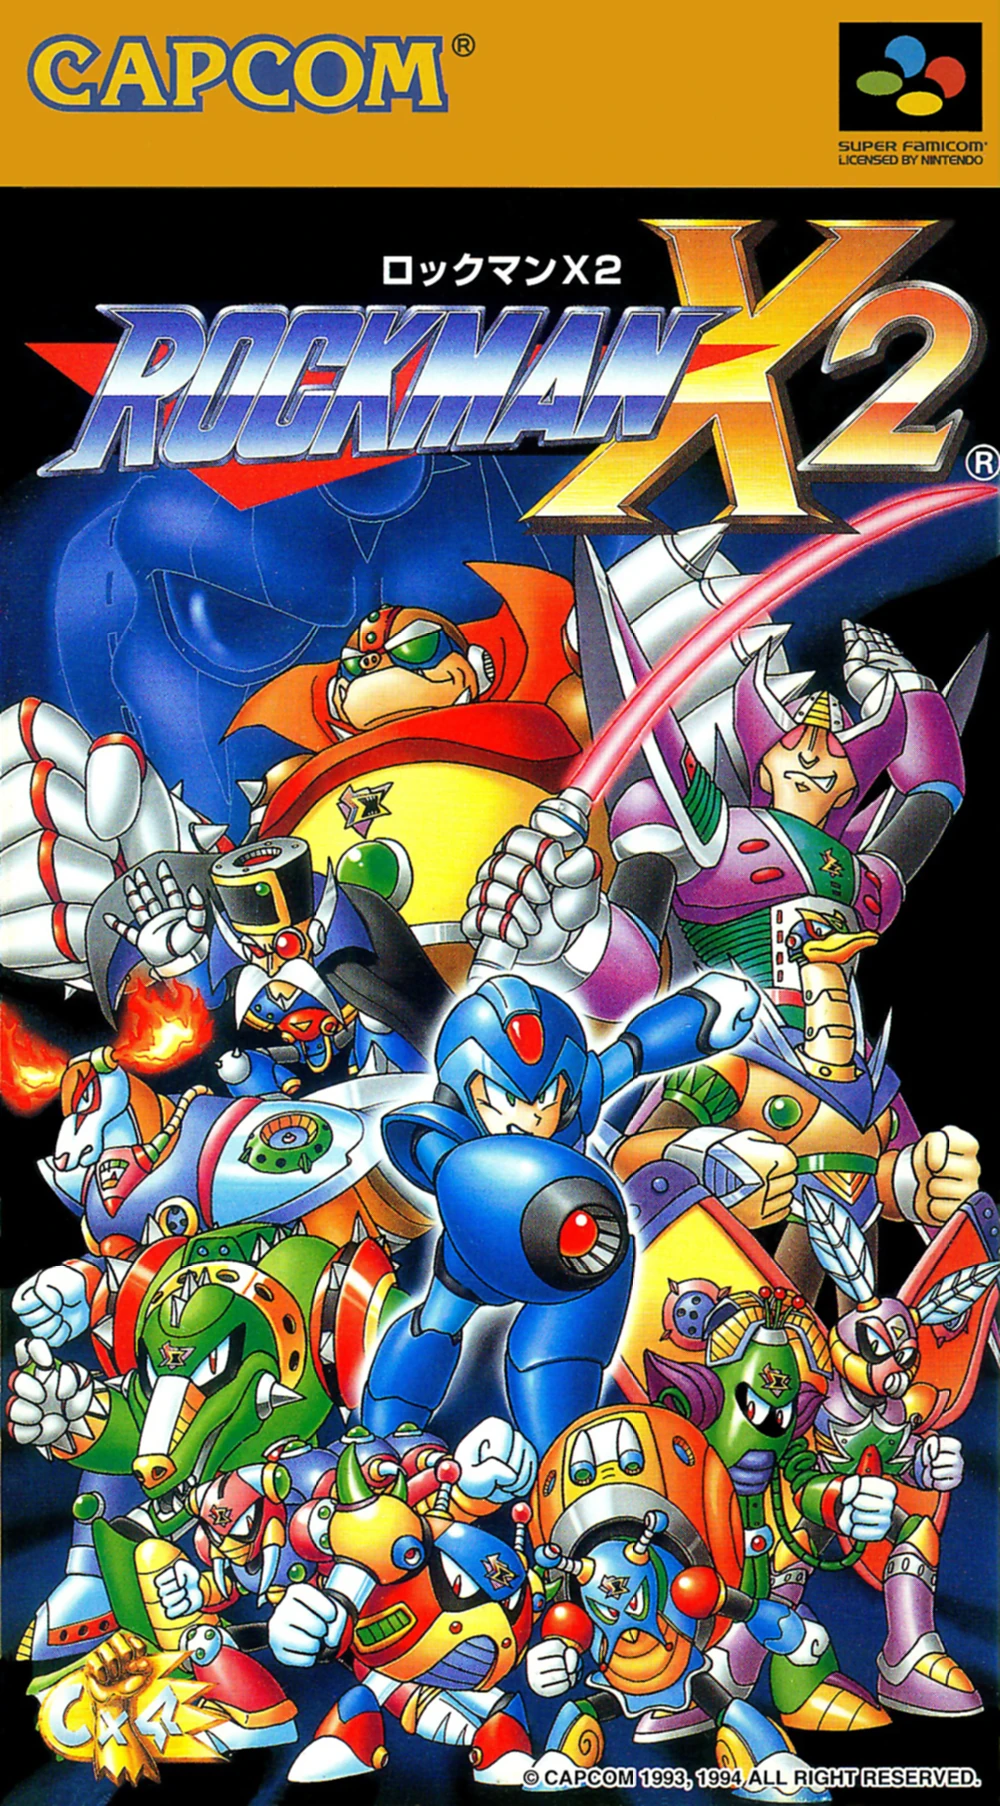
\includegraphics[height=5cm]{figures/X2/Rockman_X2_Box_Art.png}
	\end{subfigure}
	\caption{Cover art for the American and Japanese version of the game.}
\end{figure}


\section{Main plot}
Six months after Sigma's defeat by X, mavericks are still posing a threat to mankind and reploids. Maverick Hunters are still fighting against them to restore peace, but the heavy losses undergone during the first revolution has reduced the number of available Hunters to a quarter of their original value~\cite{Xcoll1:Manual_X2}. Furthermore in later periods maverick attacks have been increasing in number and many Maverick Hunter bases have been attacked and destroyed, despite the original number of reploids joining Sigma wasn't very high. What makes the situation even worse is that by analyzing defeated mavericks, scientists have found a special chip bearing Sigma's insignia, installed at the moment of their creation responsible for them going maverick. After some research, the  Maverick Hunters manage to locate the factory where these mavericks are created and X, alongside the 17th Unit, begins its attack on the facility.
\begin{figure}[htp]
	\centering
	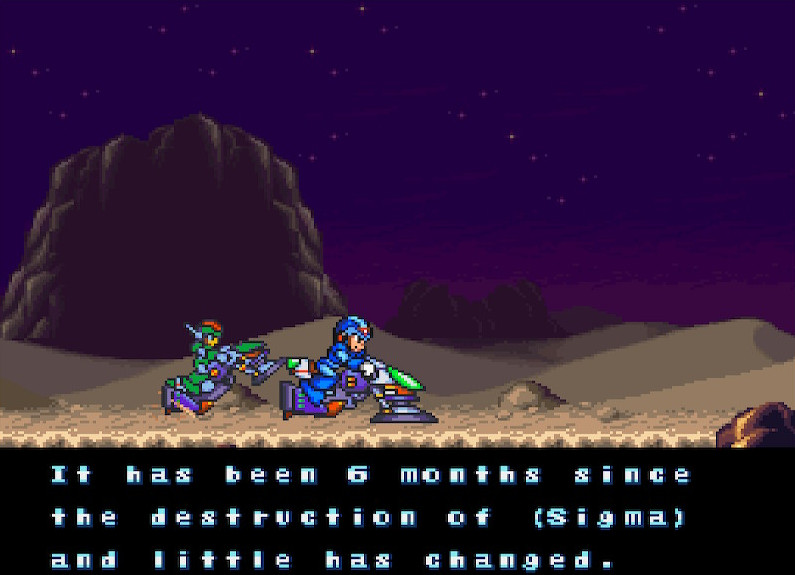
\includegraphics[height=4cm]{figures/X2/story_1.jpg}
	\caption {X attacking the maverick factory}
\end{figure}
It is during this operation that Mega Man X2 starts: after a harsh fight outside the facility, X manages to enter and destroy it, but only after having dealt with one of the giant mechaniloid CF-0 produced in the factory. After the fight the scene moves away from X, revealing three figures in the shadow, observing X's movement on a monitor and commenting on how he could pose a threat to their plans. Although they do not seem to fear him they recognize his strength and the fact that he could interfere in their plans, for which they're in hurry, and decide to let him fight with their eight SA-class maverick subordinates to gather time and complete their scheme.

\begin{figure}[htp]
	\centering
	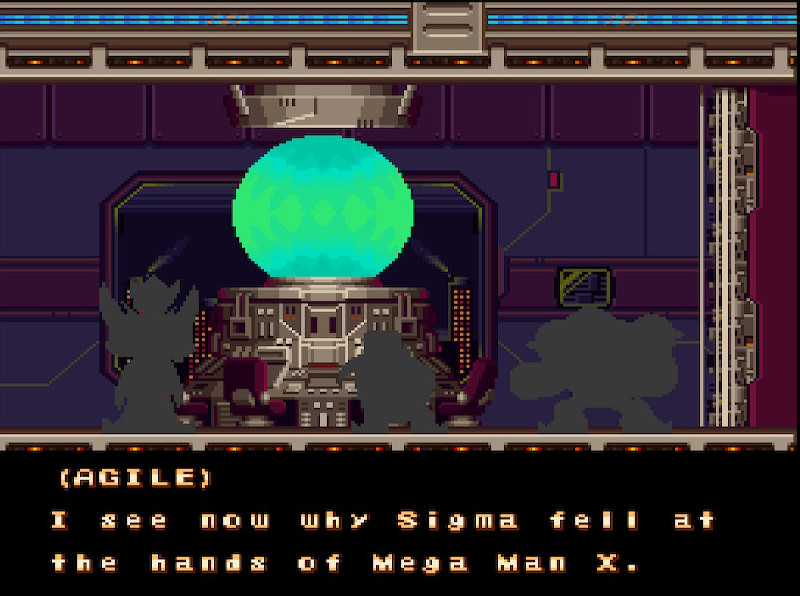
\includegraphics[height=4cm]{figures/X2/story_2.jpg}
	\caption {The X-Hunters realizing X's strength}.
\end{figure}
X, however, proves himself to be far superior with respect to the three figure's expectations, disposing of mavericks at a faster rate than imagined. This leads the three figures to come out from the shadows and face X directly, both slowing down X and attempting to eliminate him by themselves. The three contact than the Maverick Hunter headquarters and present themselves: they're Agile, Serges and Violen leaders of a group called the ``X-Hunter'' (\textit{``Counter-Hunter''} in the Japanese version) which act has a counterpart to the Maverick Hunter and aims to destroy them. The three pose a challenge X : if he manages to locate and fight all of them in a one-vs-one fight, for each of them X defeats he will receive one of Zero's body parts they had previously retrieved and repaired. These, together with Zero's control parts recovered and preserved inside the M.H. headquarters, could allow him to resurrect his friend. For here the story can take two paths, depending weather the player manages to locate and defeat all the X-Hunter or not:
If X gather all Zero's parts Dr.~Cain will begin his reparation, and in the meanwhile he will also locate the X-Hunter fortress; on the other hand, should X miss at least one of them, they will storm Dr.~Cain's laboratory and steal all Zero's component, control circuit included, to revive him as a Maverick, but also leaving a trace pointing to their headquarter, which in both case results to be located in the north pole.

Once reached the X-Hunter fortress, X infiltrates inside and fights once more against the X-Hunter, only this time their objective is to effectively dispose of him and not to slow down. This translates in them recurring to their full power and all means to take down X: Violen challenges X as Neo Violen, a more powerful form of him, Serges tries to stop him by recurring to his Serges Tank and finally Agile by using the Agile Flyer; however none of them succeed in the plan and are all defeated by X. Unluckily for X though, X-Hunter plan was in the end completed as a reborn Sigma contact X while the fortress he is in start exploding, and challenges him to a fight in the Central computer, a location already visited by X while facing mavericks sent by the X-Hunter. Once X reaches the location, two events can occur based on the outcome of Zero's quest.

Shouldn't X have recovered all Zero's part, allowing the X-Hunter to steal all the remaining one, he will find Sigma, with his new body, alongside a repaired Zero which however doesn't show any sign of consciousness, as he attacks X as soon as Sigma orders him to do it. Only after being defeated by X Zero regains his consciousness, apologizes to X for all the trouble he has caused and decides to help X by opening a passage for him to reach Sigma.

If instead X managed to recover all Zero's parts when reaching the Central Computer he would find instead Sigma alongside a black replica of Zero, which Sigma intends to use against X. Luckily the real Zero appears, easily destroying his replica and leaving Sigma surprised in finding out Zero decided to size with X. After this dialogue Sigma retreats, but Zero opens up a passage for X to chase him down.

\begin{figure}[htp]
	\centering
	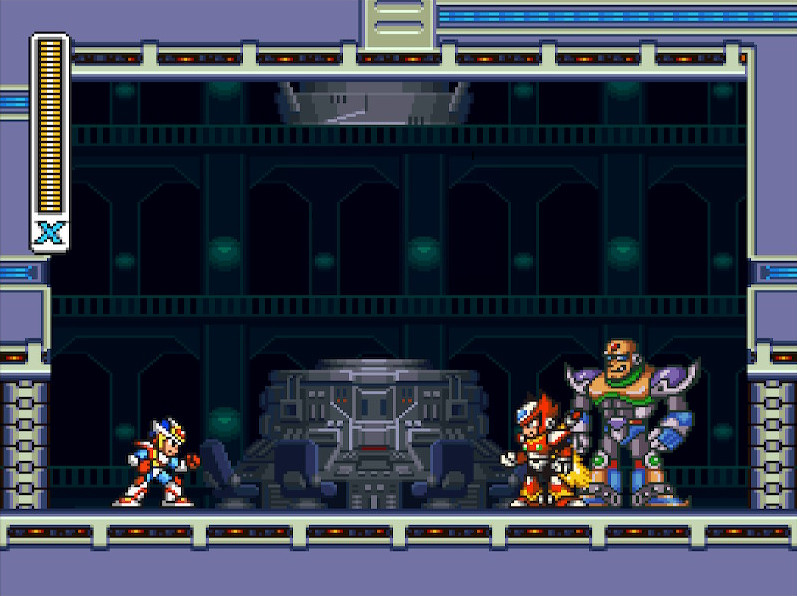
\includegraphics[height=4cm]{figures/X2/story_3_2.jpg}
	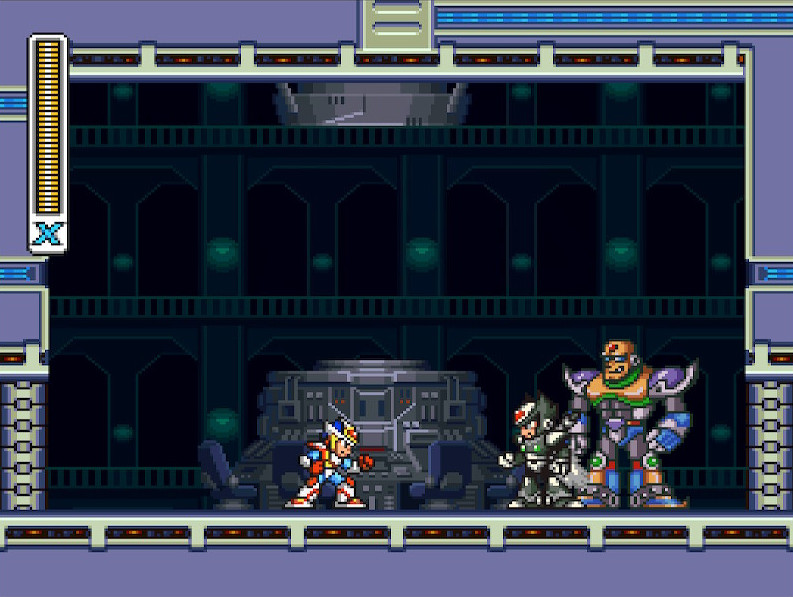
\includegraphics[height=4cm]{figures/X2/story_3.jpg}
	\caption{X against Sigma and Zero/Fake Zero.}
\end{figure}

Whatever the two previous events happen, in the end X will always reach the final confrontation with Sigma, reborn in a new body and ready to face X once more. As in the previous game, however, X manages to destroy Sigma's new body but this time only to reveal Sigma's true form: the Sigma virus. Sigma appears in fact not anymore as an actual reploid, but rather as a materialized virus with a consciousness. After a long battle X finally manages to defeat Sigma again, which disappears but before making his final warning. This time however, instead of blaming X for the failure of his plans, Sigma warns X that he will always manage to match his power, whatever the level his. Nevertheless, one thing seems to bother Sigma while disappearing, this being Zero siding with X. Sigma, in fact, was sure beyond any limit that Zero would have followed him, almost as it was his destiny.

After Sigma's defeat, X and Zero reunite together near a seaside. Here X ponders again on the reason for his fight, on why he has such incredible power within him and, more importantly, if he will ever be capable of admiring realized the dream of a world where humans and reploids coexist and that Dr.~Light dreamed of.

\begin{figure}[htp]
	\centering
	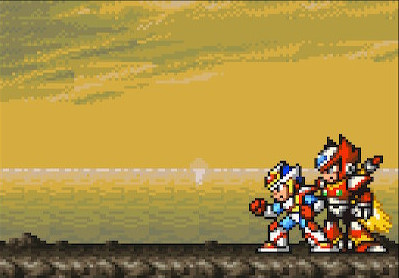
\includegraphics[height=4cm]{figures/X2/Ending.jpg}
	\caption{Game's ending scene}
\end{figure}
\section{Main Characters}

\subsection{X}

\begin{figure}[htp]
	\centering
	
\includegraphics[height=4cm]{figures/X2/X.png}
	\caption{X as he appears in X2.}
\end{figure}

X (see also chap.~[\ref{char:X}])  is Dr.~Light's last creation and the basis on which Dr.~Cain developed all reploids, although X's technology cannot be fully understood even with the knowledge of the time. When Sigma began his revolution against humanity X stood up and fought him, putting a halt to Sigma's plans and bringing peace to the world. Thanks to this, X was promoted leader of the 17th Elite Unit, which he belongs to and was previously lead by Sigma himself and Zero, a close friend of X which sacrificed himself to save him, but his Hunter rank have remained unchanged although some people have started noticing that X's hidden potential could even surpass the abilities of SA-ranked Hunter.

Despite his incredible power, X remains a kindhearted person which refuse to believe violence is the only solution to the maverick problems, and the turmoil caused by his kind spirit and the need to fight to protect innocent is something very few people understand\cite{Xcoll1:Manual_X2}.

\subsection{Zero}

\begin{figure}[htp]
	\centering
	
\includegraphics[height=5cm]{figures/X1/Zero_X1.png}
	
\includegraphics[height=5cm]{figures/X2/Hunter_stages/Zero.png}
	\caption{Zero as he appeared in X1 and how appears from X2 onward.}
\end{figure}

Zero (chap.~[\ref{char:Zero}]) is an SA-ranked Maverick Hunter under the 17th Elite unit and is X's best friend as well as only one of few people who could truly understand X's feelings. During Sigma' war he was appointed leader of the Maverick Hunter and led the others against Sigma. However near the end of the conflict Zero was forced to detonate his energy core to protect his friend X, dying in the process. Luckily his control chip remained intact and was brought to the Maverick Hunter headquarters where they reside during the event of this game.

Similar to X, however, Zero's body is far too complex to be repaired even by a scientist of Dr.~Cain's level, but not for X-Hunter's scientist Serges, who not only manages to repair Zero's body but even to upgrade it in order to revive him as a Maverick\cite{wayback:X2_resources} (even succeeding depending on which ending the player achieve). Whether to be Serges or Dr.~Cain (with Serges' rebuilt parts) to rebuild him, Zero makes his return at the end of the game, where he either challenges X or destroys his copy, and opens the to Sigma for X. He is later seen during the end, gazing at the sea near his friend.


\subsection{Dr.~Cain}
\begin{figure}[htp]
	\centering
	
\includegraphics[height=5cm]{figures/Characters/Char_Cain_X2.png}
	\caption{Dr~Cain.}
\end{figure}
Dr.~Cain (see also [\ref{char:Cain}]) is the greatest expert in robotics of the 22$^nd$ century\cite{Xcoll1:Manual_X2}. By using Dr.~Light's schematics and X's help, he solely managed to transform robots of his times, by introducing reploids, robots perfectly capable of thinking and acting autonomously as well as showing emotions. This, however, also led to the appearance of mavericks, not last Sigma which, by chance, was Dr.~Cain 's greatest creation. In the present Dr.~Cain acts as the founder of Maverick Hunter, also covering a position on its high vertex as well as playing a supportive role in the Maverick haunt, as the X2 games show. Here, in fact, Dr.~Cain coordinates X's operation from remote, locating in the end the X-Hunter's base for the final attacks. He also works to restore and repair Zero, but only when provided with all already-restored parts X recovers from all the X-Hunter.

\subsection{X-Hunters}
\begin{figure}[htp]
	\centering
	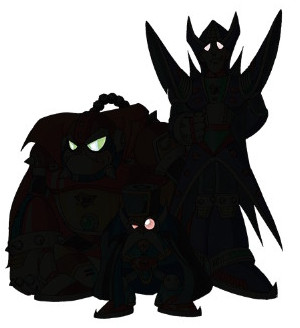
\includegraphics[height=5cm]{figures/X2/Enemies/X_Hunters.jpg}
	\caption{The X-Hunters.}
\end{figure}

After Sigma's defeat by the hand of X, it was believed mavericks attacks would cease, as there was no leader to command them. But this was not the case. Although at first the loss of their leader may have led the maverick army to a series of losses against the more organized, even if weakened Maverick Hunter, not so much time had to pass before a new head would appear to lead the rebellion. Only this time instead of a single one, three reploids took charge of the army: a group called the X-Hunter.

Composed by three incredibly strong reploids, Agile, Serges and Violen, this group takes the lead of Sigma's army, and re-organized it in order to bring on Sigma's plan from where it stopped. The first step consists in the creation of more maverick troops in order to reinforce the army. To do so a reploid factory is conquered and altered in order to implant special chips inside produced reploids to brainwash them into loyal maverick soldiers. Furthermore inside the factory giant reploids CF-0 are also built to increase even more their military potential.

The second, and more important step, in X-Hunter plans, is the revival of both Zero and Sigma. This plan, however, requires a large amount of time to be completed, as only Serges is the one capable of building a new body for Sigma and repairing Zero's parts they recovered. Beside time, the other limiting factor to the plan is the missing of Zero's own control circuit, the only component saved by Maverick Hunter and now stored in their headquarters. To gain time to complete their project, the three decide to deploy the eight SA-ranked mavericks they have to hit strategic objectives and slow down Hunter's operations. They however underestimate X's strength, as he disposes of deployed maverick at a much faster rate their plan proceed, which force them to intervene in first person and, more importantly, to use Zero's part they restored  as prize to force X into a fight, with the risk of losing a key factor of their plan. Depending on how the game proceed, they can either be all defeated, which leads them to retreat into their fortress and hurry to complete their plan by creating a fake Zero replica, or survive the fight with X, giving them the chance to attack the Hunter's headquarter while X isn't there and stole all Zero's components, to fully resurrect him as a maverick, but also leaving a trace for X to follow them to their hideout.

In both cases, X manages to find the X-Hunter headquarters and begins his attack. To stop him, the three decide to fight him each one on their own and use all their available equipment to surpass him in strength. However none of the three succeeds, as all of them in the end are defeated and destroyed by X.


\section{Game Mechanics}
Being a direct sequel of \textit{Mega Man X}, \textit{Mega Man X2} reuses almost every game mechanics present in the first title, while also bringing some new feature to the gameplay:
\begin{itemize}
	\item Dashing: X now has the ability to dash from the start. However this ability can be further enhanced, allowing for air-dashing.
	\item Stage Interactions: stages now no longer interact between them, hence beating a level now doesn't grant any advantages in another one.
	\item X-Hunter challenges: Once the second boss is defeated, the three X-Hunter will begin appearing inside remaining levels. X-Hunter movements can be seen in the map screen as soon as the player returns to it, where the player will see the remaining Hunter teleporting from one stage to another. Once inside a stage the X-Hunter can be challenged inside a secret room X can meet while traveling the level, but which normally are inaccessible. For each Hunter defeated X will receive a Zero part to resurrect his friend, meanwhile skipping the fight will cause the X-Hunter to flee forever, losing the chance to get the part for good. Finally should the player get a game-over, or enter and exit an already-beaten level, it will trigger X-Hunter movement across remaining levels.
	\item Ride Chaser: In a certain stage X will gain access to the Ride Chaser, a motorcycle capable of traveling at high speed but that cannot be stopped. This vehicle moves autonomously in the direction the player is facing, can jump and dash forward but cannot be stopped and will explode if it makes contact with a wall, leaving the player on foot. Differently from a Ride Armor, the Ride Chaser does not protect X while driving, so X will take full damage when hit by an enemy.
	\item New Ride Armor: This game features an upgraded Ride Armor from the previous game. This new version is controlled just as the precedent, but can also perform a charged dash attack, by keeping the fire button pressed, and hover for a short amount of time by pressing the jump button.
\end{itemize}

\section{Weapons}\label{X2:sub_weapon}
Here are now listed all sub-weapons available inside \textit{Mega Man X2}~\cite{wiki:X_weapons}

\subsection{\includegraphics[width=12px, height=10px]{figures/X2/weapons/C_Hunter.png} Crystal Hunter}\label{Crystal_Hunter}
Crystal Hunter shoots a glob of liquid which crystallizes small enemies that come in contact with it. Crystallized enemies cannot move and, if they were flying, they will fall on the ground. X can use the formed crystal as a platform to stand on, or dash through it to instantly shatter the crystal and the enemy inside it. Enemies destroyed in this way will always drop a health capsule of random size. When charged, this weapon will cause the screen to distort for a little and slow down the time, resulting in everything on screen (X included) to move slower. This weapon is obtained by defeating Crystal Snail~[\ref{boss:Crystal_snail}]

\begin{figure}[htp]
	\centering
	\begin{subfigure}{0.39\linewidth}
		\includegraphics[width=\linewidth]{figures/X2/weapons/C_Hunter_1.png}	
	\end{subfigure}
	\begin{subfigure}{0.275\linewidth}
		\includegraphics[width=\linewidth]{figures/X2/weapons/C_Hunter_2.png}	
	\end{subfigure}
	\caption{Crystal Hunter sub-weapon and trapped enemy.}
\end{figure}

\subsection{
\includegraphics[width=12px, height=10px]{figures/X2/weapons/B_splash.png} Bubble Splash}\label{Bubble_splash}
Bubble Splash is the weapon obtained by defeating Bubble Crab~[\ref{boss:Bubble_crab}]. When used it will fire a stream of bubbles which slightly curve upward as they move and pop if they make contact with enemies.  The number of bubbles fired depends on how much the fire button is pressed: a light pressure will cause few bubbles to spawn, while a heavier pressure will cause more to spawn, up to seven in total~\cite{wiki:Bubble_splash}. Keeping the fire button pressed will make the weapon fire continuously, making new bubbles appear as soon as previous ones pop. When charged this weapon will create several bubbles which will orbit around X and damage enemies which come in contact with it. However, the orbitals bubble will keep draining X's energy, only to disappear once it has been all depleted. Furthermore, since keeping the fire button pressed is required to charge up the weapon, X will keep shooting bubbles in the process, consuming energy while doing so. 

Underwater Bubble Splash will behave slightly differently: fired bubbles will curve upward much faster and, when charged, the weapon will allow X to jump much higher than normal.

\begin{figure}[htp]
	\centering
	\begin{subfigure}{0.4\linewidth}
		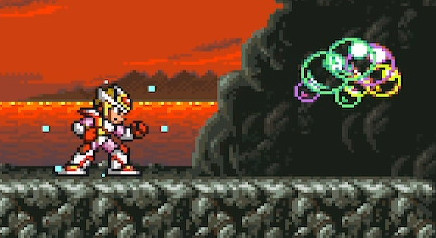
\includegraphics[width=\linewidth]{figures/X2/weapons/B_splash_1.jpg}	
	\end{subfigure}
	\begin{subfigure}{0.275\linewidth}
		
\includegraphics[width=\linewidth]{figures/X2/weapons/B_splash_2.jpg}	
	\end{subfigure}
	\caption{Bubble splash normal fire and charged version.}
\end{figure}

\subsection{
\includegraphics[width=12px, height=10px]{figures/X2/weapons/S_shot.png} Silk Shot}\label{Silk_shot}
By defeating Morph Moth~[\ref{boss:Morph_moth}] X will acquire the Silk Shot. When used X will launch a hunk of garbage in front of him, while when charged X will draw to him a huge mass of scraps, which remains attached to the X buster acting as a shield as long as the fire button remains pressed, only to be released and explode when the button is released.
\begin{figure}[htp]
	\begin{subfigure}{\linewidth}
		\centering
		
\includegraphics[width=0.4\linewidth]{figures/X2/weapons/S_shot_1.png}	
		
\includegraphics[width=0.4\linewidth]{figures/X2/weapons/S_shot_2.png}	
		\caption{Crystals}	
	\end{subfigure}
	\begin{subfigure}{\linewidth}
		\centering
		
\includegraphics[width=0.4\linewidth]{figures/X2/weapons/S_shot_3.png}	
		
\includegraphics[width=0.4\linewidth]{figures/X2/weapons/S_shot_4.png}	
		\caption{Leafs}
	\end{subfigure}
\end{figure}
\begin{figure}
	\ContinuedFloat
	\centering
	\begin{subfigure}{\linewidth}
		\centering
		
\includegraphics[width=0.4\linewidth]{figures/X2/weapons/S_shot_5.png}	
		
\includegraphics[width=0.4\linewidth]{figures/X2/weapons/S_shot_6.png}	
		\caption{Rocks}	
	\end{subfigure}
	\begin{subfigure}{\linewidth}
		\centering
		
\includegraphics[width=0.4\linewidth]{figures/X2/weapons/S_shot_7.png}	
		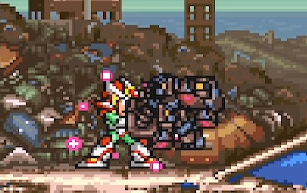
\includegraphics[width=0.4\linewidth]{figures/X2/weapons/S_shot_8.png}	
		\caption{Scraps}
	\end{subfigure}
	\caption{Silk Shot attack types in normal and charged versions.}
\end{figure}


This weapon is probably one of the most gimmicky of the entire series due to its two features. The first, and most important, one is the fact that damage dealt and projectile type fired by the weapon will change depending on the stage it is used in (charged version remain almost unchanged, save for the type of material drawn), according to following scheme~\cite{wiki:Silk_shot}:
\begin{itemize}
	\item In the \textbf{Energen crystal mine} stage the weapon will shoot a crystal shard which moves in the direction X is facing while bouncing on the floor. Upon making contact with a wall the crystal explodes in an X shape
	\item In the \textbf{Weather Control stage} the weapon will fire a pile of leaves  which float upwards. This is the weakest version of Silk Shot.
	\item In the \textbf{Volcanic Zone} and \textbf{Deep Sea base} the weapon will fire a rock projectile, which will bounce on the ground once before exploding.
	\item In all remaining stages the weapon will fire a metal scrap, which explodes as soon as it touches a surface, ground included.
\end{itemize}

The second feature of this weapon is its ability to draw health and energy capsules when its charged shot is used inside special rooms in some specific stages (see section~\ref{sec:refill}).


\subsection{
\includegraphics[width=12px, height=10px]{figures/X2/weapons/S_wheel.png} Spin Wheel}\label{Spinning_wheel}
When using the Spin Wheel, X fires a buzz saw blade which falls on the ground and then crawls along the floor, continuously damaging enemies which come in contact with it until the blade disappears or the enemy is destroyed. In the latter case the blade will then restart moving forward until it disappears. The saw can also destroy certain blocks and terrains, to open new passages, but only one blade per time can be on screen. When charged, X will release a blade which, instead of moving forward, will split into eight energy bolts traveling in all directions. Bolts pass through obstacles and enemies, dealing damages while also maintaining destructive properties of the uncharged version. This weapon is obtained after defeating Wheel Gator~[\ref{boss:Wheel_gator}].

\begin{figure}[htp]
	\centering
	\begin{subfigure}{0.4\linewidth}
		
\includegraphics[width=\linewidth]{figures/X2/weapons/S_wheel_1.png}	
	\end{subfigure}
	\begin{subfigure}{0.3\linewidth}
		\centering
		
\includegraphics[width=\linewidth]{figures/X2/weapons/S_wheel_2.png}	
	\end{subfigure}
	\caption{Spin Wheel normal and charged version.}
\end{figure}

\subsection{
\includegraphics[width=12px, height=10px]{figures/X2/weapons/S_slicer.png} Sonic Slicer}\label{Sonic_slicer}
After defeating Overdrive Ostrich~[\ref{boss:Overdrive_ostrich}] X will gain access to the Sonic Slicer. This weapon fires a spinning blade which travels horizontally at high speed and ricochets on walls with increasing angle of reflection each time, before disappearing once an enemy is hit or it goes offscreen. When charged this weapon fires five blades very close to each other upwards, which then separates and descend down becoming larger in the process.

\begin{figure}[htp]
	\centering
	\begin{subfigure}{\linewidth}
		\centering
		
\includegraphics[height=2.5cm]{figures/X2/weapons/S_slicer_1.png}	
	\end{subfigure}
	\begin{subfigure}{0.25\linewidth}
		\centering
		
\includegraphics[height=2.5cm]{figures/X2/weapons/S_slicer_2.png}	
	\end{subfigure}
	\begin{subfigure}{0.7\linewidth}
		\centering
		
\includegraphics[height=2.5cm]{figures/X2/weapons/S_slicer_3.png}	
	\end{subfigure}
	\caption{Sonic Slicer normal and charged version.}
\end{figure}

\subsection{
\includegraphics[width=12px, height=10px]{figures/X2/weapons/S_chain.png} Strike Chain}\label{Strike_chain}
When using the Strike Chain, X will release a chain with a hook at its end, which can both damage enemies which come in contact with them. How much the chain extends depends on the length the fire button is pressed: a short pressure will cause the chain to extend slightly, while a longer pressure will cause the chain to extend up to its limit. Beside dealing damage, the chain is also able to grub items from distance, enemy drops included, and if a wall is hit, it will pull X towards it. When the weapon is charged X will release a faster and longer chain, which also deals more damage. Furthermore enemies destroyed in this way will always drop an energy pickup for X. This weapon is obtained by defeating Wire Sponge~[\ref{boss:Wire_sponge}]

\begin{figure}[htp]
	\centering
	
\includegraphics[height=2.5cm]{figures/X2/weapons/S_chain_1.png}	
	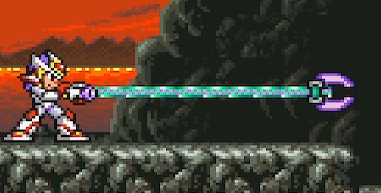
\includegraphics[height=2.5cm]{figures/X2/weapons/S_chain_2.png}	
	\caption{Strike Chain normal and charged version.}
\end{figure}
\begin{figure}[htp]
	\centering
	
\includegraphics[height=2.5cm]{figures/X2/weapons/S_chain_grub.jpg}	
	\caption{Strike Chain grab ability.}
\end{figure}

\subsection{
\includegraphics[width=12px, height=10px]{figures/X2/weapons/M_mine.png} Magnet Mine}\label{Magnet_mine}
\begin{figure}[htp]
	\centering
	\begin{subfigure}[t]{0.4\linewidth}
		
\includegraphics[width=\linewidth]{figures/X2/weapons/M_mine_1.png}	
		\caption{Normal fire}
	\end{subfigure}
	\begin{subfigure}[t]{0.4\linewidth}
		\centering
		
\includegraphics[width=\linewidth]{figures/X2/weapons/M_mine_2.png}	
		\caption{Three mines stacked onto each other.}
	\end{subfigure}
\end{figure}
\begin{figure}[htp]
	\ContinuedFloat
	\centering
	\begin{subfigure}[t]{0.4\linewidth}
		\centering
		
\includegraphics[width=\linewidth]{figures/X2/weapons/M_mine_3.png}	
		\caption{Charged version}
	\end{subfigure}
	\begin{subfigure}[t]{0.4\linewidth}
		\centering
		
\includegraphics[width=\linewidth]{figures/X2/weapons/M_mine_4.png}	
		\caption{Absorbing incoming projectiles}
	\end{subfigure}
\end{figure}
\begin{figure}[htp]
	\ContinuedFloat
	\centering
	\begin{subfigure}[t]{0.4\linewidth}
		\centering
		
\includegraphics[width=\linewidth]{figures/X2/weapons/M_mine_5.png}	
		\caption{Charged version second stage}
	\end{subfigure}
	\begin{subfigure}[t]{0.35\linewidth}
		\centering
		
\includegraphics[width=\linewidth]{figures/X2/weapons/M_mine_6.png}	
		\caption{Charged version max size}
	\end{subfigure}
	\caption{Magnet Mine sub-weapon.}
\end{figure}
Defeating Magna Centipede~[\ref{boss:Magna_centipede}] allows X to use the Magnet Mine. This weapon fires a single mine which travels at constant speed in the direction it is shot. If the mine makes contact with an enemy it explodes, but if it hits a surface it remains in place for a short time, before exploding. Once a mine attaches to a surface X can immediately fire another one, which can land on the previous one, forming a chain. There is virtually no limit on how many mines X can fire, but typically only four can be shot before the first one explodes. More importantly, the path of each mine can be controlled vertically by inputting up or down, but once a direction is given the mine will follow that direction, meaning that to make it go straight again it is necessary to keep inputting up and down.

Once charged, the weapon will release a small slow-moving black hole which can be controlled similarly to the base version (see \path{videos/X2/Charged_mine_control.mp4}). The black hole keeps moving forward, passing through obstacles and enemies (which are still damaged) and absorbing incoming projectiles, growing in size in the process up to two stages bigger, but also becoming more difficult to control.



\subsection{
\includegraphics[width=12px, height=10px]{figures/X2/weapons/S_burner.png} Speed Burner}\label{Speed_burner}
Speed Burner releases from the X-buster a pair of intertwined fireballs which travel at high speed in straight direction, disappearing once they collide with an enemy or a surface. In addition, if Speed Burner is fired while standing on the ground, it will also leave a small trace of fire along its path which deals damage to enemies too. When charged this weapon will wrap X in flames and make him dash forward at high speed, damaging enemies. When in this state X doesn't take contact damages from enemies, but he does from stage hazards like spikes. This attack can also be used in the air, allowing X to perform an air dash.

Similar to the previous game, this fire weapon behaves differently when used inside water. For the regular attack, in fact, underwater the two fireballs won't ignite, and only two small orbs (which deal very small damage) will be shot leaving behind a trail of smoke. For the charged version instead X will simply dash forward, again leaving behind a trail of smoke. When in this state X is not invincible, and will take damage if he makes contact with an enemy.

\begin{figure}[htp]
	\centering
	\begin{subfigure}[t]{0.4\linewidth}
		
\includegraphics[width=\linewidth]{figures/X2/weapons/S_burner_1.png}	
	\end{subfigure}
	\begin{subfigure}[t]{0.4\linewidth}
		\centering
		
\includegraphics[width=\linewidth]{figures/X2/weapons/S_burner_2.png}	
	\end{subfigure}
	%\end{figure}
	%\begin{figure}
	%	\ContinuedFloat
	%	\centering
	\begin{subfigure}[t]{0.4\linewidth}
		\centering
		
\includegraphics[width=\linewidth]{figures/X2/weapons/S_burner_3.png}	
	\end{subfigure}
	\begin{subfigure}[t]{0.4\linewidth}
		\centering
		
\includegraphics[width=\linewidth]{figures/X2/weapons/S_burner_4.png}	
	\end{subfigure}
	\caption{Speed Burner sub-weapon attacks outside and inside water.}
\end{figure}

\section{Second Armor}\label{X2:Armor}
Returning from the previous game Dr.~Light's capsules, each one storing a new armor part, which are scattered across four of the eight stages, although this time they are more hidden and often require a specific sub-weapon (or even other parts) in order to get access to them. Furthermore, differently from the previous game this game doesn't have any mandatory capsule, making the armor fully optional.
According to \cite{tw:second_armor}\footnote{Translation: \url{https://twitter.com/kobun20/status/1305162448878612480}}, the second armor is actually an improved version of the first one, which X had returned past first game's events. Once returned, Light's capsule analyzed armor's field data in order to upgrade it into a new armor for X.

\begin{figure}[htp]
	\centering
	\includegraphics[height=5cm]{figures/X2/X2armor.png}
	\caption{The Second Armor.}
\end{figure}

The second armor is again composed of four main parts, with the addition of a fifth, secret, one in a similar way the Hadoken was in the first game.

The Second Armor is composed by following components:
\begin{itemize}
	\item Foot parts: When equipped, these parts allow X to perform dashes, already available from the start, in the air too. However air-dashes cannot be performed if X has already dashed on the ground or if he is already dash-jumping. However Foot Parts' air dash flight distance can be extended by combining it with a charged Speed Burner. The capsule containing this power-up is hidden inside the Desert Base, behind a wall breakable only by the Spin Wheel sub-weapon.
	\begin{figure}[htp]
		
		\centering
		\includegraphics[width=0.4\linewidth]{figures/X2/Overdrive_ostrich/Ostrich_capsule.jpg}	
		\caption{Foot Parts location}
	\end{figure}	
	
	\item Body Parts: Similarly to the previous game, this power-up increases X's defense by halving all incoming damages to X. Furthermore, all damage dealt to X will also increase a special gauge which, one full, allows X to perform the \textit{Giga Crush} attack, which heavily damages all enemies on screen. 
	However the gauge doesn't refill between stages, meaning the only way to store energy is by getting hit. The capsule containing Body Parts is hidden in the Robot Junkyard stage, under a floor at the beginning of the stage breakable only with the Spin Wheel sub-weapon.
	\begin{figure}[htp]
		\centering
		\begin{subfigure}{0.4\linewidth}
			\centering
			\includegraphics[width=\linewidth]{figures/X2/Morph_moth/Moth_capsule_2.jpg}
		\end{subfigure}
		\begin{subfigure}{0.4\linewidth}
			\centering
			\includegraphics[width=\linewidth]{figures/X2/weapons/G_crush_1.png}
		\end{subfigure}
		\caption{Body Parts location and Giga Crush attack.}
	\end{figure}.
	
	
	\item Arm Parts: This upgrade allows X to use two X-buster when using a charged shot. When charging, X will be able to pass the second charge level, accumulating energy in the second Buster, up to two levels.  When the player releases the fire button, X will shoot a first charged shot (depending on the charge level reached) and will remain flashing until the fire button is pressed again, making X release a second, fully charged, shot. Most importantly, if the player releases the two charged shots in rapid succession, they can combo against all enemies, bosses included, ignoring their invincibility frame and dealing massive damage. This upgrade is stored inside Wheel Gator stage, inside a chamber accessible only via wall jumping from an opening on the roof, and can be obtained either via precise wall-jumping, by using the the Giga Crush to extend X's airborne period, by using the Strike Chain to pull X towards the wall (\path{videos/X2/Buster_capsule_chain.mp4}), or simply by using the air dash to reach the opening.
	\begin{figure}[htp]
		\centering
		\begin{subfigure}{0.4\linewidth}
			\centering
			\includegraphics[width=\linewidth]{figures/X2/Wheel_gator/Gator_capsule.jpg}
		\end{subfigure}	
		\begin{subfigure}{0.4\linewidth}	
			\includegraphics[width=\linewidth]{figures/X2/weapons/Double_shot.png}
		\end{subfigure}	
		\caption{Arm Parts location  and double charged shot.}
	\end{figure}
	
	\item Head Parts: The Head Parts allow X to use the item tracer, a radar which X can fire and will point in the direction of the closest secret in the level. Secrets pointed include hidden passages and items (such as ), heart tanks and sub-tanks, other Light's capsules and refill rooms. Despite showing an ammunition gauge, this upgrade does not use any energy. The capsule with the Head Parts is hidden in Crystal Snail's stage, at the end of a secret path found while sliding down a pit after the stage's sub-boss.
	\begin{figure}[htp]
		\centering
		\includegraphics[width=0.4\linewidth]{figures/X2/Crystal_snail/Crystal_capsule.jpg}
		\includegraphics[width=0.345\linewidth]{figures/X2/weapons/Tracer.png}
		\caption{Head Parts location and Item Tracer.}
	\end{figure}
	
	\begin{figure}[htp]
		\centering
		\includegraphics[width=0.4\linewidth]{figures/X2/Hunter_stages/Shoryuken_capsule.jpg}
		\includegraphics[width=0.335\linewidth]{figures/X2/weapons/Shoryuken.png}
		\caption{Shoryuken's capsule location and attack.}
	\end{figure}
	\item Shoryuken\label{shoryuken}: Similarly to X1's Hadoken, this secret upgrade is the prize for collecting all other power-up items (Zero's parts do NOT count). Once obtained, X will be able to perform the fire uppercut from the \textit{Street Fighter} series by inputting the command $\rightarrow$, $ \downarrow$, $\searrow$ (with X facing left) + fire button but ONLY if X is at full health and on the ground. Differently from the previous technique, however, is the fact that the damage dealt by this technique is dependent on the number of frames the attack makes contact with an enemy, meaning that a misplaced Shoryuken can fail to insta-kill bosses. To be precise, Shoryuken deals 16 damage to enemies without invincibility frame and 8 otherwise and the damage is applied every two frames, meaning that in order to kill a boss at full health (32 hit points) 5 frame of contact are needed (16 damage the first frame, than zero the second, 8 the third, than again 0 on fourth and last 8 at the fifth). 
	This upgrade can be found inside the third X-Hunter stages, at the end of a secret passage full of spikes which requires a precise air dash. In order to obtain this capsule, moreover, X has to reach it with full health (but there are no limitations on Sub Tank status).
\end{itemize}

\section{Opening Stage}
Being the first stage in the game, this level acts as a tutorial for the player to (re-)learn basic game mechanics. The stage begins with a short scene where X and other Hunters are riding their vehicles to the factory, but are attacked by a fierce resistance. X then jumps off his bike, which crashes onto an enemy, and proceeds on foot. From here the player gains X's control and can start moving. Attention must be done immediately, however, since the enemy on which the bike crashed on is still alive and will shoot X immediately. Past this first obstacle the player will enter the factory where other enemies lie ahead, such as \hyperlink{enem:Bar_Waying}{Bar Waying} which do not deal damage but use their body to block the path and require several shots to be destroyed. Traversing the factory X will find himself onto a production line, which uses conveyor belts to move manufactured mavericks from one construction bay to the other (three in total); if X get caught inside one of they bays he will receive damage, while if he pass over it the bay will simply upgrade the constructed maverick which, in case of the third and last bay, will activate and attack X. Near the end there is a mini wall-jump tutorial: a \hyperlink{enem:Slidame}{Slidame}, as soon as it detects X, will rush at the top of the room it waits and begin closing the walls in an attempt to crush X. Although not very fast, the player has to climb the wall quickly in  order to not get killed by the wall. Should instead the player fall down back to the room's bottom and the wall close it will be sufficient to return back in the stage a little, in order to reset the room as it was before, giving another chance to climb. Once reached the top of the room a small corridor awaits, ending in a deep pit which X has to jump into, as at the end a boss door awaits.

Beside enemies already cited, this level also house following enemies~\cite{wiki:X2_opening}:
\begin{itemize}
	\item \hyperlink{enem:Bar_Waying}{Bar Waying}
	\item \hyperlink{enem:Cannon_Driver}{Cannon Driver}
	\item \hyperlink{enem:Mecha-Arm}{Mecha-Arm}
	\item \hyperlink{enem:Scrambler}{Scrambler}
	\item \hyperlink{enem:Scriver}{Scriver}
	\item \hyperlink{enem:Slidame}{Slidame}
\end{itemize}

\subsection{Giant Mechaniloid CF-0}
\begin{figure}[htp]
	\centering
	\includegraphics[height=5cm]{figures/X2/Enemies/CF0.png}
	\caption{Giant Mechaniloid CF-0's artwork}
\end{figure}
Differently from the previous game, this opening stage ends in a boss fight the player has to win. The boss in question is the giant mechaniloid CF-0, an enormous robot created by the X-Hunter with the purpose of mass production and conquering cities around the world, although due its weight the movement speed is reduced to the minimum. X-Hunter' plans were however halted by Maverick Hunter's attack, which forced them to activate the only completed mechaniloid to try to stop the attack, but resulting only in its destruction by the hands of X.

Despite its size, the fight against CF-0 is relatively simple. The boss room is very big and and filled with platform at various level, connected by ladders to allow X to climb up should he fall down, and this allow X to easily dodge the two attacks this boss can perform: a spiked fist which aims at player's current position and a jump attack where CF-0 aims to land onto X. However both of these attacks can be easily avoided by keeping moving between top platforms and deals minimal damage to X. It is in fact on the upper side of the room that X should stay to damage the boss, as its only weak point is the head, which happens also to be one of the three body parts that can damage X if he makes contact with them, the other ones being CF-0's arms and feet. All the rest of its body does not deal any damage of any sort, acting like a background. Finally, and having the health bar of a boss, CF-0 takes massive damage from X's charged shot, which can destroy it in four shots.

\begin{figure}[htp]
	\centering
	\begin{subfigure}{0.5\linewidth}
		\centering
		\includegraphics[height=4cm]{figures/X2/cf_punch.jpg}
		\caption{CF-0 punching}
	\end{subfigure}
	\begin{subfigure}{0.4\linewidth}
		\centering
		\includegraphics[height=4cm]{figures/X2/cf_walk.jpg}
		\caption{CF-0 walking around}
	\end{subfigure}
	\caption{Giant Mechaniloid CF-0's attacks.}
\end{figure}

\begin{figure}[htp]
	\centering
	\includegraphics[width=0.5\linewidth]{figures/X2/map.png}
	\caption{Full map with Bosses and their locations}
\end{figure}


\section{Weather Control}
The first stage the game presents is the weather control stage. As the name suggests, the focus of the stage are weather conditions, which can change and be controlled as the stage progresses in order to affect X's mobility or enemies' behavior. The source of said weather changes is to be found in an element presented right at the beginning of the level: \hyperlink{enem:Weather_crystal}{weather crystals}. Although these items are considered enemies, they won't hurt X in any way, even if he makes contact with them. What they will do, instead, is change the weather in the portion of the level X is in, affecting X's movement and changing enemies' behavior and power. While this can only appear to be a cons, the truth is X can manipulate said enemies to obtain favorable weather to ease the stage exploration. There are a total of four crystals in the stage, each one with a default weather set which can be changed depending on the weapon X uses to hit it, according to following list~\cite{wiki:Weather_crystal}:
\begin{figure}[htp]
	\centering
	\begin{subfigure}{0.3\linewidth}
		\centering
		\includegraphics[width=\linewidth]{figures/X2/Wire_sponge/sponge_crystal_default.jpg}
		\caption{Intact crystal}
	\end{subfigure}
	\begin{subfigure}{0.3\linewidth}
		\centering
		\includegraphics[width=\linewidth]{figures/X2/Wire_sponge/sponge_crystal_cloud.jpg}		
		\caption{Cloudy}
	\end{subfigure}
	\begin{subfigure}{0.3\linewidth}
		\centering
		\includegraphics[width=\linewidth]{figures/X2/Wire_sponge/sponge_crystal_sun.jpg}
		\caption{Sunny}
	\end{subfigure}
	\begin{subfigure}{0.3\linewidth}	
		\centering
		\includegraphics[width=\linewidth]{figures/X2/Wire_sponge/sponge_crystal_rain.jpg}\\
		\caption{Rainy}
	\end{subfigure}
	\begin{subfigure}{0.3\linewidth}
		\centering
		\includegraphics[width=\linewidth]{figures/X2/Wire_sponge/sponge_crystal_fog.jpg}
		\caption{Foggy}	
	\end{subfigure}
	\begin{subfigure}{0.3\linewidth}
		\centering
		\includegraphics[width=\linewidth]{figures/X2/Wire_sponge/sponge_crystal_broken.jpg}
		\caption{Broken crystal}	
	\end{subfigure}
	\caption{Different states of weather condition and crystals.}
\end{figure}
\begin{itemize}
	\item \textbf{Cloudy weather}: Obtained hitting the crystal with the Strike Chain weapon (the crystal turns yellow). In this state all enemies are active and \hyperlink{enem:Sky_farmer}{sky farmers} plant \hyperlink{enem:Sabottein}{sabotteins}, which only grow half-size.
	\item \textbf{Warm/Sunny weather}: Obtained by hitting the crystal with the Speed Burner (the crystal turns orange). In this state all enemies are active, but \hyperlink{enem:Croak_hopper}{croak hoppers} will overheat and explode, while planted \hyperlink{enem:Sabottein}{sabotteins} will growth to their full size.
	\item \textbf{Rainy weather}: Obtained by hitting the crystal with the Bubble Splash (the crystal turns cyan). In this state \hyperlink{enem:Croak_hopper}{croak hoppers} will actively move for the stage instead of staying in place, while planted \hyperlink{enem:Sky_farmer}{sky farmers} will release \hyperlink{enem:Rightod}{rightods} to chase X. \hyperlink{enem:Sole_solar}{sole solars} will instead remain deactivated. Finally in rainy weather a constant, inverse, speed is applied to X while moving, resulting in a slower walking and running speed, as well as a shorter jump distance.
	\item \textbf{Foggy weather}: Obtained by using the Crystal Hunter on the crystal (it turns purple/black). In this state all enemies are deactivated.
\end{itemize}

Should the player destroy a crystal, weather conditions for the stage's portion will be set at random.

The first crystal the player finds is near the beginning of the level, in a very straightforward section with only some enemies to stop X and that ends with a second weather crystal, opening to the second part of the level. Here floating platforms will move up and down over a spiked pit, and X has to move from one to another paying attention as platforms are taller than wider, meaning the best way to stay on them is by wall-jumping. The main difficulty in this section is given by the default weather set, which is the rain that will reduce X's jump distance, making it harder for the player to pass from one platform to the next one. The third section is very similar to the first one, only with more enemies and spiked pits. Here are the last two weather crystals, which will activate different enemies as the player proceeds. Once this part has been passed, a climbing section awaits, with platforms with enemies on top and connected by ladders ending in a corridor which leads to the boss door.

Following enemies occupy the stage~\cite{wiki:weather_control}
\begin{itemize}
	\item \hyperlink{enem:Aclanda}{Aclanda}
	\item \hyperlink{enem:Croak_hopper}{Croak Hopper}
	\item \hyperlink{enem:Rightod}{Rightod}
	\item \hyperlink{enem:Sabottein}{Sabottein}
	\item \hyperlink{enem:Scriver}{Scriver}
	\item \hyperlink{enem:Sky_farmer}{Sky Farmer}
	\item \hyperlink{enem:Sole_solar}{Sole Solar}
	\item \hyperlink{enem:Weather_crystal}{Weather Crystal}
\end{itemize}


\subsection{Heart Tank}
The Heart Tank is hidden immediately at the beginning of the stage. By climbing the leftmost wall of the beginning room, the player will find a small entrance in the top corner with the Heart Tank inside it.

\begin{figure}[htp]
	\centering
	\begin{subfigure}{0.4\linewidth}
		\centering
		\includegraphics[width=\linewidth]{figures/X2/Wire_sponge/Sponge_heart.jpg}
		\caption{Heart Tank location.}
	\end{subfigure}
	\begin{subfigure}{0.4\linewidth}
		\centering
		\includegraphics[width=\linewidth]{figures/X2/Wire_sponge/Sponge_Hunter_room.jpg}
		\caption{X-Hunter room location.}
	\end{subfigure}
	\caption{Locations for the Heart Tank and X-Hunters room in the Weather Control Center}
\end{figure}
\subsection{X-Hunter' room}
When reaching the elevator section, if the player manages to make X sneak under the elevator a new path will open, leading to the X-Hunter room

\subsection{Sub Tank}
In the rain section, if instead of proceeding by platforming the player uses the first one to jump onto the wall on the right (where the second crystal is found) and climb it, it will reach a new path over the default one made of logs separated into two main platforms. At the end of the second one is where the Sub Tank resides.  
\begin{figure}[htp]
	\centering
	\includegraphics[width=0.4\linewidth]{figures/X2/Wire_sponge/Sponge_tank.jpg}
	\caption{Sub Tank location.}
\end{figure}

\subsection{Wire Sponge}\label{boss:Wire_sponge}
\begin{figure}[htp]
	\centering
	\includegraphics[height=5cm]{figures/X2/Wire_sponge/Wire_Sponge.png}
	\caption{Wire Sponge's artwork~\cite{book:MMX_Complete_art}}
\end{figure}
Wire Sponge (the ``Little Forest Demon''~\cite{book:MMX_Complete_art}) was a sponge cucumber-based SA-class Maverick manufactured inside one of Sigma's factories although born from an accident. Because of a design mistake, in fact, Wire Sponge was built with a personality disorder which made him childish, cheerful and easily amused, with the love for dancing and playing. Although this personality was not tailed for army, Wire Sponge's strength  and violence was uncontested, and X-Hunter put that in use by making him conquer the weather control center which he uses as his own playground, changing the weather as he please~\cite{wiki:wire_sponge},\cite{wayback:X2_resources}.

In battle, Wire Sponge mainly attacks by swinging his chord, the Strinke Chain in various ways to damage X.
\begin{figure}[htp]
	\centering	
	\begin{minipage}{0.4\linewidth}		
		\begin{subfigure}{\linewidth}
			\centering
			\includegraphics[width=\linewidth]{figures/X2/Wire_sponge/Sponge_spin.png}
			\caption{Spinning the chain}
		\end{subfigure}
		\begin{subfigure}{\linewidth}
			\centering
			\includegraphics[width=\linewidth]{figures/X2/Wire_sponge/Sponge_pull.jpg}
			\caption{Being pulled to the wall}
		\end{subfigure}
	\end{minipage}
	\begin{minipage}{0.4\linewidth}		
		\begin{subfigure}{\linewidth}
			\centering
			\includegraphics[width=\linewidth]{figures/X2/Wire_sponge/Sponge_hang.jpg}
			\caption{Hanging and launching seeds.}
		\end{subfigure}
	\end{minipage}
\end{figure}
When Wire Sponge spins his chain he will deflect all incoming projectiles, so attacking while in this state is useless. After spinning the chain, Wire Sponge will almost always attack by throwing it at X and, if the chain hits a wall, he will be pulled towards it. Other times Wire sponge will instead throw the chain on the ceiling and start climbing it, while firing seeds from his head aiming at X. When a seed hits a wall or the floor (not the roof, of which the seed will ricochet on) it will grow into a spiked vine which damages X on contact. These spikes can be destroyed by any weapon and doing it is a suggested action, since after four vines are planted Wire Sponge will drop down~\cite{rta:x2} terminating his attack which leaves him very open for damages, so the longer he performs it the better. Finally once Wire Sponge's health drops below 10 points he will start using his desperation moves. With this move his flower becomes a lightning rod from which he will make lightning fall in the room but they can be easily avoided as they fall at the same distance every time and never near the boss himself, so staying close is a good strategy to avoid taking damage. However once this attack is performed Wire Sponge will become charged with electricity which will increase his damage output.
\begin{figure}[htp]
	\ContinuedFloat
	\centering
	\begin{subfigure}{\linewidth}
		\centering
		\includegraphics[width=0.4\linewidth]{figures/X2/Wire_sponge/Sponge_phase2.jpg}
		\includegraphics[width=0.4\linewidth]{figures/X2/Wire_sponge/Sponge_DM.jpg}
		\caption{Charging and releasing his desperation move}
	\end{subfigure}
	\begin{subfigure}{0.4\linewidth}
		\centering
		\includegraphics[width=\linewidth]{figures/X2/Wire_sponge/Sponge_charged.jpg}
		\caption{Powered up by electricity}
	\end{subfigure}
	\begin{subfigure}{0.35\linewidth}
		\centering
		\includegraphics[width=\linewidth]{figures/X2/Wire_sponge/Sponge_cut.jpg}
		\caption{Cut in half.}
	\end{subfigure}
	
	\caption{Wire Sponge's attacks.}
\end{figure}

Wire Sponge is often considered an easy boss due the long time he makes himself vulnerable when he hangs from the ceiling and the fact that all his other attacks are easy to dodge. This makes fighting him with only the buster relatively safe, also since his main weakness, the Sonic Slicer doesn't do much more to him than increased damage (and a different animation when it is used to defeat him).

According to in-game data, Wire Sponge possesses a power of 6400 rp and a speed of 4800 rp, and upon defeating him X will gain access to the Strike Chain~[\ref{Strike_chain}].
\begin{table}[htp]
	\centering
	\begin{tabular}[h]{l c c}
		
		\toprule
		\multicolumn{2}{c}{Health}  & 32\\
		\midrule
		\multicolumn{1}{c}{Attack} & \multicolumn{1}{c}{Damage}& \multicolumn{1}{c}{Damage-electrified}\\
		Contact & 5 & 7\\
		Strike Chain & 2 & 4\\
		Seed/Vines& 2&-\\
		Lightnings & 2&-\\
		\bottomrule
	\end{tabular}
	\caption{Wire Sponge's attack's damages~\cite{wiki:wire_sponge}}
\end{table}

\section{Robot Junkyard}
As the name suggests, the Robot Junkyard stage takes place inside a scrapyard where old robots are demolished.

The beginning of the stage corresponds to the junkyard's entrance. From here it is already possible to see how most of the enemies in the level will present themselves: most of them will be, in fact, old robots ready to be destroyed or repaired in some way, that will attack X as he comes closer. The beginning of the stage consists in a long corridor full with enemies and a magnet on the roof which pulls metal upwards thus enhancing X's jump capabilities, although this little bonus is totally useless, as there are no pits in this section. Continuing in the level the player will face the first of two sub-boss: entering inside the capsule room will in fact trigger the door closure and free from the capsule itself a \hyperlink{miniboss:Pararoid_S-38}{Pararoid S-38} which will possess and \hyperlink{miniboss:Old_robot}{Old Robot}. This enemy is heavily armored and X's attack will bounce off it unless aimed at its center, the only spot which can take damage. Old Robot's main attacks consist in moving toward X by performing small jumps, making a big jump in the air and diving onto X and occasionally firing junk projectiles. Although the sub-boss itself may not appear as dangerous as other ones, the real difficulty of the battle comes from its possible-endless duration. As the Old Robot is destroyed (easily done by using a charged Spin Wheel, if available) the Pararoid S-38 will exit the robot's body and immediately dive into the ground in order to resurrect another one, basically resetting all player's progress in the boss fight. In order to avoid this a well-aimed Charges Shot or, even better, Speed Burner are sufficient to defeat the small insect and open the exit door.

Once outside the sub-boss rooms a long ladder will bring X deeper in the stage, until reaching another corridor, similar to the first one met, awaits. However here magnets will work in the opposite way respect the first one, reducing X's jump height, but again this can be totally ignored, as no platforming is required in the section. At the end of the corridor a ladder awaits to bring X a level lower in the stage inside a room where a second combination of  \hyperlink{miniboss:Paraloid_S-38}{Pararoid S-38} and \hyperlink{miniboss:Old_robot}{Old Robot} has to be fought again as second sub-boss of the stage to access, upon its defeat, to the last stage's corridor before the boss room.

Following enemies appears in the stage~\cite{wiki:Robot_Junkyard}:
\begin{itemize}
	
	\item \hyperlink {enem:Cannon_Driver}{Cannon Driver}
	\item \hyperlink {enem:Disk_Boy_08}{Disk Boy 08}
	\item \hyperlink {enem:Garakuta_Robot}{Garakuta Robot} 
	\item \hyperlink {enem:Hanged_Reploid}{Hanged Reploid}
	\item \hyperlink {enem:Pararoid_R-5}{Pararoid R-5}
	\item \hyperlink {miniboss:Pararoid_S-38}{Pararoid S-38} and \hyperlink{miniboss:Old_robot}{Old Robot}
	\item \hyperlink {enem:Pararoid_V-1}{Pararoid V-1}
\end{itemize}


\subsection{Heart Tank}
Near the beginning of the stage, before entering the junkyard facility the player will spot a \hyperlink {enem:Disk_Boy_08}{Disk Boy 08} on top of a platform. By trapping it with the Crystal Hunter it is possible to create a higher platform for X to jump on and, from the top of it, dash jumping onto the upper part of the junkyard entrance where a life up and the heart tank are hidden. Alternatively if the player is capable of performing a \emph{Neon Jump} (see section \ref{Neon_jump} for more details) it can use it to reach the upper level without having to obtain the Crystal Hunter weapon first, as it is possible to see in file \path{videos/X2/Moth_heart_double_jump.mp4}.

\begin{figure}[htp]
	\centering
	\begin{subfigure}{0.305\linewidth}
		\centering
		\includegraphics[width=\linewidth]{figures/X2/Morph_moth/Moth_heart_1.jpg}	
		\caption{}
	\end{subfigure}
	\begin{subfigure}{0.4\linewidth}
		\centering
		\includegraphics[width=\linewidth]{figures/X2/Morph_moth/Moth_heart_2.jpg}
		\caption{}	
	\end{subfigure}
	\caption{Heart Tank location: from (a) it is necessary to reach the upper-right wall in order to reach (b). Using a crystal Hunter on the enemy which stands on where X is is the intended way.}
\end{figure}


\subsection{Light's Capsule}\label{X2:Body_parts}
In the first magnetized roof section, near its end if the player uses the Item Tracer power-up from the helmet the radar will point at a specific position on the floor. If the player releases in that spot a Spin Wheel (normal or charged), the blade will start digging in the terrain, opening a new path which leads to the armor capsule holding the body upgrade. The item tracer is not mandatory, as experienced players can open the passage directly.
\begin{figure}[htp]
	\centering
	\begin{subfigure}{0.4\linewidth}
		\centering
		\includegraphics[width=\linewidth]{figures/X2/Morph_moth/Moth_capsule_1.jpg}	
		\caption{}
	\end{subfigure}
	\begin{subfigure}{0.4\linewidth}
		\centering
		\includegraphics[width=\linewidth]{figures/X2/Morph_moth/Moth_capsule_2.jpg}
		\caption{}	
	\end{subfigure}
	\caption{Armor Capsule's location. From (a) the Spin Wheel will open a passage up to (b).}
\end{figure}



\subsection{X-Hunter' room}
In the long ladder section if instead of dropping down directly X jumps to the right he will find a corridor leading to the Hunter's room.

\subsection{Morph Moth}\label{boss:Morph_moth}
\begin{figure}[htp]
	\centering
	\includegraphics[height=5cm]{figures/X2/Morph_moth/Morph_Moth.png}
\end{figure}
Morph Moth was a mysterious reploids with an unknown past and affiliation. An experimental prototype, Morph Moth was built with the special capability  of powering himself up by absorbing scraps, in order to evolve from his cocoon form to the adulthood~\cite{wiki:Morph_moth},\cite{wayback:X2_resources}. This particular feature caught Sigma' interests, which enrolled him into his army only to be deployed by the X's Hunter during their revolution. The plan was to use Moth's special ability in controlling scraps to resurrect and create new mavericks for their army. However Morph Moth never showed any particular interest in his work.

The battle against Morph Moth is split into two phases, the cocoon form being the first. While in this state Moth will perform three attacks cyclically. The first attack is the Scrap Scatter, where Morph Moth swings at increasing speed, scattering scraps around, only to fall down when the speed is high enough to break the string. At this point Moth will begin to attack with his Dash Scrap Scatter, moving underground from one side of the arena to the other while scattering more scraps as he goes. Finally he will re-hang himself to the ceiling and start performing his Scrap Absorption attack, absorbing scrap in clockwise or counterclockwise ways at high speed, increasing in size in the meanwhile. 

\begin{figure}[htp]
	\centering
	\begin{subfigure}{0.3\linewidth}
		\centering
		\includegraphics[width=\linewidth]{figures/X2/Morph_moth/Moth_1.jpg}
	\end{subfigure}
	\begin{subfigure}{0.3\linewidth}
		\centering
		\includegraphics[width=\linewidth]{figures/X2/Morph_moth/Moth_2.jpg}
	\end{subfigure}
	\begin{subfigure}{0.3\linewidth}
		\centering
		\includegraphics[width=\linewidth]{figures/X2/Morph_moth/Moth_3.jpg}
	\end{subfigure}
	\vspace{2pt}
	\begin{subfigure}{0.3\linewidth}	
		\centering
		\includegraphics[width=\linewidth]{figures/X2/Morph_moth/Moth_4.jpg}
	\end{subfigure}
	\begin{subfigure}{0.3\linewidth}
		\centering
		\includegraphics[width=\linewidth]{figures/X2/Morph_moth/Moth_5.jpg}	
	\end{subfigure}
	\begin{subfigure}{0.3\linewidth}
		\centering
		\includegraphics[width=\linewidth]{figures/X2/Morph_moth/Moth_6.jpg}
	\end{subfigure}
	\caption{Different stages of Morph Moth's growth.}
\end{figure}

The second phase of the boss fight can be triggered in two ways. The first (and often seen) one is by bringing Moth's health below 75\%, while the second one can be achieved by letting him absorb enough scraps to achieve full-size (if left performing his attacks, the player will note that Moth's cocoon will increase in size). One one of these conditions are met, Morph Moth will exit the arena destroying the ceiling, to reappear shortly after in his Moth form. In this second phase Morph Moth has only two attacks he'll perform while flying around: the first one is the Phosphorescent Powder, where he will start gliding down leaving behind a trace of scales which slowly descends and damage X on contact; the second one is the Beam attack, where he fires a powerful beam aiming at player's position~\cite{book:Compendium}.


\begin{figure}[htp]
	\centering
	\begin{subfigure}{0.4\linewidth}
		\centering
		\includegraphics[height=3.5cm]{figures/X2/Morph_moth/Moth_swing.jpg}
		\caption{Swinging}
	\end{subfigure}
	\begin{subfigure}{0.5\linewidth}
		\centering
		\includegraphics[height=3.5cm]{figures/X2/Morph_moth/Moth_underground.jpg}
		\caption{Dashing underground}
	\end{subfigure}
	\begin{subfigure}{0.4\linewidth}
		\centering
		\includegraphics[width=\linewidth]{figures/X2/Morph_moth/Moth_powder.jpg}
		\caption{Phosphorescent Powder}
	\end{subfigure}
	\begin{subfigure}{0.4\linewidth}
		\centering
		\includegraphics[height=5cm]{figures/X2/Morph_moth/Moth_beam.png}
		\caption{Beam}
	\end{subfigure}
	\begin{subfigure}{\linewidth}
		\centering
		\includegraphics[height=4cm]{figures/X2/Morph_moth/Moth_burn.jpg}
		\includegraphics[height=4cm]{figures/X2/Morph_moth/Moth_hurt.jpg}
		\caption{Burnt in cocoon form and hurt in Moth form}.
	\end{subfigure}
	\caption{Morph Moth's attacks.}
\end{figure}


Battling Morph Moth without taking much damage can be hard. In his cocoon form the scraps he tosses around will be thrown randomly, so quick reflexes are needed to avoid them, while to dodge the absorption attack quick and precise wall jumps have to be made in order to jump from one side of the arena to the other, while also avoiding to land on the boss. In the second phase, instead, Moth will continuously perform attacks, alternating between the two he has, which can be difficult to dodge: the scales cover a wide area, while the beam comes out fast and aims at the player, which could find difficult to dodge if already dealing in avoiding the scales. Furthermore in this phase Moth's attack power is increased, meaning  he can deal many damages in a short amount of time. Moth's weakness is the Speed Burner, which will set him on fire dealing heavy damages and stunning him, but it does not have any other effects, meaning the boss will keep performing all his attacks in order without any limitation.

Also labeled the ``\textit{Fallen Angel from the Island of Dreams}''~\cite{book:MMX_Complete_art}, Morph Moth possesses a power equal to 3200 rp and a speed of 8800 rp. Once defeated X will gain access to the Silk Shot (\ref{Silk_shot}) which, ironically, is able to destroy most enemies found in the stage in one hit, sub-bosses included.


\begin{table}[htp]
	\centering
	\begin{tabular}[h]{l c}
		
		\toprule
		\multicolumn{1}{c}{Health}  & 32 \\
		\midrule
		\multicolumn{1}{c}{Attack} & \multicolumn{1}{c}{Damage}\\
		Contact - Cocoon & 4 \\
		Contact - Moth& 8\\
		Scraps (any) & 2\\
		Phosphorescent Powder& 2\\
		Beam & 2\\
		\bottomrule
	\end{tabular}
	\caption{Morph Moth's attack's damages~\cite{wiki:Morph_moth}}
\end{table}

\section{Volcanic Zone}
The Volcanic Zone Stage is, among all other stages, the one which will test the player's ability in climbing and wall jumping~\cite{stratwiki:Volcanic_zone}. 

The stage's beginning is relatively easy, as no enemies are present except for a single \hyperlink{enem:Beetron}{Beetron}, which will move up and down until it matches X’s same vertical height. At that point it will ram into X and, if it hits a breakable wall, Beetron will destroy it, opening a passage but also destroying itself in the process. Besides opening new passages X can also stand onto Beetrons, as they have a platform on top.

Whether X enters the volcano from the top or by breaking the bottom-left wall (in this case the player will find a small passage with healing items) the second stage's section takes place inside the active volcano. here as X reaches a metallic floor the screen will start shaking. From that moment the lava will begin rising, leaving as the only escape option climbing up to the volcano's top. To do this the player must be very quick and precise in wall jumping, as the exit conduit is not regular but presents several narrowing and ledges which require continuous moving from one wall to the other. Once reached the top the lava will continue to erupt upwards, not following X anymore.

The third section is an outside one, where the player has to platform between rock pillars, which will begin collapsing into the lava as soon as X touches them. At the section's end a second Beetron can be found, which can be used to open one of the two blocked passages (one above and one below the main one) for the second indoor section. Here there is first some platforming to do between collapsing pillars onto a lava pool and then a final climb part. This time there is no lava chasing X,  but the section is full of pipes which constantly emits gas that can be set on fire when a \hyperlink{enem:Morgun}{Morgun} enemy lands near a pipe. The fire lasts for some time and deals heavy damage to X, so disposing of these enemies is suggested. The gas itself does not damage X, so standing in front of it is safe.

Once exited from the second volcano, by going a little further to the right the player will find the boss door.

Following enemies appears in the level~\cite{wiki:Volcanic_zone}
\begin{itemize}
	\item \hyperlink{enem:Bar_Waying}{Bar Waying}
	\item \hyperlink{enem:Barite_Lastar}{Barite Lastar}
	\item \hyperlink{enem:Beetron}{Beetron}
	\item \hyperlink{enem:Morgun}{Morgun}
\end{itemize}


\subsection{Sub Tank}
Right at the beginning of the stage if the player manages to reach the entrance to the volcano without destroying the Beetron, and from there jump on to the platform this enemies carry on, the Beetron will move backwards until it reaches a hidden zone on the top left of the map, where the Sub Tank resides. 

\begin{figure}[htp]
	\centering
	\includegraphics[height=2.5cm]{figures/X2/Flame_stag/Stag_tank_2.jpg}
	\includegraphics[height=2.5cm]{figures/X2/Flame_stag/Stag_tank_3.jpg}
	\includegraphics[height=2.5cm]{figures/X2/Flame_stag/Stag_tank.png}	
	\caption{Sub Tank location.}
\end{figure}


\subsection{Heart Tank}
While escaping from the lava in the first volcano the player will immediately notice the Heart Tank, in plain sight on one of the many narrows while climbing. Reaching this collectible can be difficult, not only due to the lava chasing the player, which will kill X if he is too slow, but also for the Bar Waying enemy which will act as a wall, slowing down the process to get it even further. The best way to get this item is to climb as fast as possible and dispose of the Bar Waying as soon as he appears by using weapons such as Spin Wheel, Magnet Mine or Silk Shot.
\begin{figure}[htp]
	\centering
	\includegraphics[height=5cm]{figures/X2/Flame_stag/Stag_heart.png}
	\caption{Heart Tank location.}
\end{figure}

\subsection{X-Hunter' room}
When entering the second volcano, if the player uses the second Beetron to destroy the upper wall two possible passages will open: by going down the player will return to the main route and continue in the level, while going up the player will find the X-Hunter's room.
\begin{figure}[htp]
	\centering
	\includegraphics[height=5cm]{figures/X2/Flame_stag/Stag_Hunter_room.png}
	\caption{X-Hunter' room location location.}
\end{figure}


\subsection{Flame Stag}\label{boss:Flame_stag}
\begin{figure}[htp]
	\centering
	\includegraphics[height=5cm]{figures/X2/Flame_stag/Flame_Stag.png}
	\caption{Flame Stag's artwork as in \cite{book:MMX_Complete_art}}
\end{figure}
Flame Stag once belonged to the 17$^{th}$ Elite Unit, where he fought alongside his friend Boomer Kuwanger.  When the rebellion began the two friends defected together, but Flame Stag became missing shortly after, whereas his friend ended up as shown in sec.~\ref{boss:Boomer_Kuwanger}. Six Months later his mysterious disappearance, Flame Stag reappeared, aiming to cause the Volcanic zone to erupt, obscuring the sun with the ashes and giving start to a new ice age. If his plan is somehow connected with X-Hunter activities is unknown.

Also known as the ``\textit{Heat Knuckle Champion}''~\cite{book:MMX_Complete_art}, Flame Stags stays faithful to his nickname and the animal he is based on by fighting with fast fire-based melee attacks in rapid succession. He will often begin the fight by performing his triangular kick attack to rapidly climb the arena's wall (which for this battle is much taller, similar to Morph Moth's one) and chasing X if he tries to climb them to avoid him. Should X instead stay on the ground Stag will perform only few jumps and then come down, where he will perform one of his remaining two attacks, these being the Speed Burner in projectile mode, where he shoots two fireball projectiles the first one which slightly descends and the second one which rises and can also climb walls, and the Speed Burner in Body Blow mode, where Flame Stag dash towards the player covered in fire and, if it hits, it will launch X in the air with a powerful uppercut. This attack also leaves behind a trail of fire which also deals damage. Finally, as most bosses of the game, if Flame Stag drops below under 50\% of health he will activate his last resort, in this case being the Super Mode. While in this state (which lasts for the all duration of the fight) Flame Stag's flame turns blue, corresponding to an increase of movement and attack speed as well as the addition of another attack following the uppercut, which consists of slamming X onto the ground after sending him fly with the first attack.

\begin{figure}[htp]
	\centering
	\begin{subfigure}{0.4\linewidth}
		\centering
		\includegraphics[height=4cm]{figures/X2/Flame_stag/Stag_triangle.png}
		\caption{Triangle Kick}
	\end{subfigure}
	\begin{subfigure}{0.4\linewidth}
		\centering
		\includegraphics[height=4cm]{figures/X2/Flame_stag/Stag_phase_2.png}
		\caption{Super Mode activation}
	\end{subfigure}
	\begin{subfigure}{0.45\linewidth}
		\centering
		\includegraphics[height= 2.25cm]{figures/X2/Flame_stag/Stag_projectile.png}
		\caption{Speed Burner Projectile}
	\end{subfigure}
	\begin{subfigure}{0.45\linewidth}
		\centering
		\includegraphics[height=2.25cm]{figures/X2/Flame_stag/Stag_dash.png}
		\caption{Speed Burner Dash}
	\end{subfigure}
	
\end{figure}
\begin{figure}
	\ContinuedFloat
	\centering
	\begin{subfigure}[t]{0.4\linewidth}
		\centering
		\includegraphics[height=5cm]{figures/X2/Flame_stag/Stag_uppercut.png}
		\caption{Uppercut from Speed Burner}
	\end{subfigure}
	\begin{subfigure}[t]{0.4\linewidth}
		\centering
		\includegraphics[height=5cm]{figures/X2/Flame_stag/Stag_descend.png}
		\caption{Slamming X onto the ground}.
	\end{subfigure}
	\caption{Flame Stag's attacks.}
\end{figure}

Despite his fast attack, all Flame Stag's attacks can be avoided relatively easily. Staying on the ground ensures him to almost never perform his triangular kick, and by dash-jumping off the walls allow to easily avoid all remaining attacks. Moreover to ease the fight even more Flame Stag possess not one but two weapons which deal him increased damages, these being the Sonic Slicer and the Bubble Splash, although only the last one is considered to be is main weakness since, beside the augmented damage, stun him and completely reset his attack pattern. This can be exploited to make Stag fall into a loop where he shoots the Speed Burner Projectiles, the player dodge them by wall-jumping and hit him with the Bubble Splash, which forces him to repeat the projectile attack, as file \path{videos/X2/Flame_Stag_loop.mp4} shows.

According to in-game data, Flame Stag possesses a power of 3600 rp and a speed of 7000 rp and once defeated X will gain access to the Speed Burner (\ref{Speed_burner}).
\begin{table}[htp]
	\centering
	\begin{tabular}[h]{l c}
		
		\toprule
		\multicolumn{1}{c}{Health}  & 32 \\
		\midrule
		\multicolumn{1}{c}{Attack} & \multicolumn{1}{c}{Damage}\\
		Contact & 2 \\
		Speed Burner- projectile& 2\\
		Speed Burner - dash& 3\\
		Speed Burner - trail& 2\\
		Speed Burner - Uppercut& 3\\
		Super mode combo & 2+5\\
		\bottomrule
	\end{tabular}
	\caption{Flame Stag's attack's damages~\cite{wiki:Flame_stag}}
\end{table}
\section{Central Computer}
The Central Computer Stage is probably one of the most difficult stage to travel due to dangers that it stores and that come in various forms, sometimes even as insta-kill traps. This stage has as its focus the stealth action, requiring X to proceed while avoiding searchlights to no trigger alarms. Avoiding being spotted is not mandatory, but triggering the alarm will activate more enemies to attack X, making it more difficult to proceed in the stage while keeping high the health level.

The first part of the stage is filled with searchlights. Here X has to proceed avoiding getting spotted, by hiding behind some background walls which block the light, but they become smaller and harder to use as the stage progresses. If the alarm triggers \hyperlink{enem:Blecker}{Blecker} enemies in the area will activate, dropping down and start shooting X, while also deactivating bridges causing more pits to appear. After proceeding deeper in the stage spotlights will disappear leaving place to another danger: \hyperlink{enem:Installer}{Installers}. These enemies are big moving blocks which will start moving as soon as X approaches them, moving into a predefined configuration and then staying in position for as long as they are on-screen. These enemies are totally invincible (safe for purple-shaded one) and, without caution, can close the player into a death trap very quickly. The section itself is not very long but the player should not relax too much, since as soon as it enters the next room the first sub-boss of the stage will appear: the \hyperlink{miniboss:Chop_Register}{Chop Register}. This miniboss, a 3D wireframe sword, can be difficult to approach at first, especially without knowing its weak point. In order to defeat the boss, in fact, the player has to attack the handle which is the only weak point, as the blade is completely invincible. The problem to face is that, most of the time, the blade will be pointed towards X to attack him, hence making hitting the handle an harder task, which is also made even harder by the fact in some occasion the blade will swing very quickly up and down, to deflect all projectiles X has shot it. The best way to deal with this boss is by having something that can one-shot him immediately as it appears, in order to avoid fighting it at all. A Giga Crush attack, or a well placed charged Sonic Slicer (ensuring that all projectiles hit the handle in the rising phase) will destroy the sub-boss immediately, as it is possible to see in file \path{videos/X2/Centipede_Chop_Register_oneshot.mp4}

After defeating the miniboss, the second part of the stage will open. Here spotlights return, only this time X has to avoid them while sliding down a wall, with hiding spot coming out from said walls. Once finished the descent X will reach a large room, where blocks will start falling from the roof. These blocks will solidify  as they reach the floor, becoming part of it and changing the room's layout. Here, if X got caught by the searchlight previously, the alarm will trigger speeding up the block's fall process and making harder to avoid damages. Also in this room a scanner will appear homing to X's position to analyze him and empower the subsequent miniboss, should X got caught. While avoiding it is rather simple with the alarm off, falling blocks can make this task harder as they slow down X if he gets hit, giving time to the radar to reach for him. As said previously, passed this small section another miniboss awaits, the \hyperlink{miniboss:Raider_Killer}{Raider Killer}. This enemy has different attack pattern and damages, depending on how many times the scanner managed to scan X, up to four in total. The upgrades regard only its offensive, and partially defensive, capabilities, but they does not impact on the total health it has. To dispose of him the Speed Burner is the suggested weapon, dealing him increased damage.

Defeated the last miniboss, a final corridor divides X from the boss' door. In this last section the alarm will always trigger, not matter what, causing \hyperlink{enem:Blecker}{Blecker} to drop down and attack, bridges to fall and open bottomless pit and also \hyperlink{enem:Installer}{Installer} to fall, to push X down the pits. If the player manages to avoid all these dangers, at the corridor's end it will reach the boss' door.

Following enemies populate the stage~\cite{wiki:Central_computer}:
\begin{itemize}
	\item \hyperlink{enem:Barrier_Attacker}{Barrier Attacker}
	\item \hyperlink{enem:Barite_Lastar}{Barite Lastar}
	\item \hyperlink{enem:Blecker}{Blecker}
	\item \hyperlink{miniboss:Chop_Register}{Chop Register}
	\item \hyperlink{enem:Installer}{Installer}
	\item \hyperlink{miniboss:Raider_Killer}{Raider Killer}
	\item \hyperlink{enem:Scrambler}{Scrambler}
\end{itemize}

\subsection{Heart Tank}
\begin{figure}[htp]
	\centering
	\includegraphics[height=4cm]{figures/X2/Magna_centipede/Centipede_heart_1.png}
	\includegraphics[height=4cm]{figures/X2/Magna_centipede/Centipede_heart_2.png}
	\caption{Heart Tank location. By not activating the Blecker, it is possible to reach the opening on the roof.}
\end{figure}
After the first searchlight section the player can notice an opening on the roof, which normally is not reachable by simply jumping. Here if the player has managed to avoid triggering the alarm a Blecker can be found near the left wall, allowing X to start wall-jumping onto it and subsequently reaching the opening where the Heart Tank is. Alternatively, should the player be able to perform a Neon Jump (sec. \ref{Neon_jump}), it is possible to reach the opening even if the alarm was triggered, as shown in the file \path{videos/X2/Centipede_heart_double_jump.mp4}

\subsection{Sub Tank}
Passing the first Installer's sections, immediately before the first sub-boss room the player can notice another opening on the roof, similar to the one leading to the Heart Tank. This time however there is no way to reach via normal jumping, as no Blecker is present to provide help. Instead what is needed to reach the opening is a combination of the Foot Parts, the Buster Parts and the Speed Burner, in order to perform a dash-jump from the left ledge (the higher one, under where the last Installer can be found) and extend the airborne period with a charged Speed Burner, making possible to reach the right wall (which is shortly lower) and start wall-jumping up to reach the room with the Sub-Tank (file \path{videos/X2/Centipede_Centipede_tank_speed_burner.mp4} gives a visual clue on how to perform such maneuver). Alternatively a Neon Jump can be performed here similarly to what was done for the Heart Tank to reach the opening, as shown in file \path{videos/X2/Centipede_tank_double_jump.mp4}

\begin{figure}[htp]
	\centering
	\includegraphics[height=4cm]{figures/X2/Magna_centipede/Centipede_tank_1.png}
	\includegraphics[height=4cm]{figures/X2/Magna_centipede/Centipede_tank.png}
	\caption{Sub Tank location.}
\end{figure}

\subsection{X-Hunters' room}
\begin{figure}[htp]
	\centering
	\includegraphics[height=4cm]{figures/X2/Magna_centipede/Centipede_Hunter_room.png}
	\caption{X-Hunters room location.}
\end{figure}
Inside the large room, past the second spotlight section and before the Raider Killer sub-boss, is where the X-Hunter room can be found. While to reach it is easy by words, as the door to enter it is located at the bottom right corner of said room, below the passage to the sub-boss, reaching it can be difficult, mainly due the falling blocks that change the room's layout. If, in fact, it happens for a block to fall in front of the door, it is possible for it to completely block the access, thus preventing from fighting the eventual boss. 

\subsection{Magna Centipede}\label{boss:Magna_centipede}
\begin{figure}[htp]
	\centering
	\includegraphics[height=5cm]{figures/X2/Magna_centipede/Magna_Centipede.png}
	\caption{Magna Centipede's artwork - \cite{book:MMX_Complete_art}}
\end{figure}
Magna Centipede was once a Maverick Hunter belonging to the Special 0$^{th}$ Unit, also known as the ``\textit{Shinobi}'' unit. During the first Maverick revolution he fought against Sigma as a Maverick Hunter but was captured while on duty and brainwashed~\cite{wayback:X2_resources}. Turned into a Maverick loyal to Sigma, Centipede became a cold-hearted and emotionless assassin (which worth him the title of ``Crimson Assassin''~\cite{book:MMX_Complete_art}) which followed every order given to him, even destroying his old comrades. Due to his blind obedience X-Hunter entrusted him with an important mission: to capture the Central Computer and use it to spread the Maverick Virus all over the world.
\begin{figure}[htp]
	\centering
	\begin{subfigure}{0.4\linewidth}
		\centering
		\includegraphics[height=4cm]{figures/X2/Magna_centipede/Centipede_shuriken.png}
		\caption{Shuriken}
	\end{subfigure}
	\begin{subfigure}{0.4\linewidth}
		\centering
		\includegraphics[height=4cm]{figures/X2/Magna_centipede/Centipede_injection.png}
		\caption{Maverick Virus}
	\end{subfigure}
	\begin{subfigure}{\linewidth}
		\centering
		\includegraphics[height= 4cm]{figures/X2/Magna_centipede/Centipede_magnet.png}
		\caption{Magnet Mine}
	\end{subfigure}
	\begin{subfigure}{0.4\linewidth}
		\centering
		\includegraphics[height=4cm]{figures/X2/Magna_centipede/Centipede_teleport.png}
		\caption{Teleporting away}
	\end{subfigure}
	\begin{subfigure}{0.4\linewidth}
		\centering
		\includegraphics[height=4cm]{figures/X2/Magna_centipede/Centipede_no_tail.png}
		\caption{Broken Tail}
	\end{subfigure}
	\caption{Magna Centipede's attacks.}	
\end{figure}
Being a ninja-type Hunter, battling with Magna Centipede cannot be easy, especially if underestimated, as a bad move can rapidly change the battle's course and snowball into a defeat. The first problem to deal with is Magna Centipede's high mobility, as he will often teleport in the arena, moving from one corner to the other (both lower and upper, in the latter case reappearing upside-down) and sometimes even multiple times to trick the player into wasting an attack. Beside the mobility, Centipede disposed of three main weapons, one deadlier than the other.

His most basic attack consists in throwing three shuriken (even multiple times) which follow a curved trajectory with different height. Next there is his Magnet Mine attack, which sees Centipede splitting his tail and sending the fragments toward X. Fragments (two at the beginning and three when on low health) orbit around X for a while, halting his shots in the meanwhile, only to close onto him shortly after. Before closing the gap, however, the tail's pieces will halt shortly, giving the player the chance to escape in the free direction and to avoid the hit. Finally there is Centipede's most dangerous attack which, although by itself doesn't deal any damage, can drastically change the battle's outcome: the Maverick Virus injection. During the fight, in fact, Magna Centipede will begin to draw X near him with great force (it is possible to avoid getting caught if X is far enough from the boss) and, once caught, will begin injecting the virus in X, debilitating him more and more for the rest of the battle. It is, however, possible to escape from Centipede's grasp by mashing any button. The real problem about this attack is that Centipede will use it regularly, so the chance of escaping from hit reduces as the fight progresses. Even worse, Centipede is able to accumulate virus effects at every injection up to four times, past which no more effect will take place, although no more are needed since after four injections X's ability will be almost totally debilitated, and the win chances with them. The virus effect injected by Magna Centipede are always the same and in the same order, and are the following~\cite{wiki:Magna_centipede}:
\begin{itemize}
	\item The first injection will disable all forms of charged shots.
	\item The second injection will block X from shooting more than one projectile at the time.
	\item The third injection will reduce the dash distance by a lot.
	\item The final injection will greatly reduce the jump height.
\end{itemize}

Should the player find out Magna Centipede's weakness, the whole fight becomes trivial. Should, in fact, X hit even only one time Magne Centipede with a Silk Shot, this would cause his tail to shatter, disabling both the Magnet Mine and Maverick Virus attacks, and leaving Centipede with the only option to teleport and attack with shuriken. This trivializes the fight, especially also due the fact that Silk Shot's metal scraps are thrown diagonally, making it the perfect weapon to hit Centipede while on the roof.
\begin{table}[htp]
	\centering
	\begin{tabular}[h]{l c}
		\toprule
		\multicolumn{1}{c}{Health}  & 32 \\
		\midrule
		\multicolumn{1}{c}{Attack} & \multicolumn{1}{c}{Damage}\\
		Contact & 4 \\
		Shuriken & 3\\
		Magnet Mine& 3\\
		Maverick Virus (1) & \multicolumn{1}{l}{0, disable charged shot}\\
		Maverick Virus (2) & \multicolumn{1}{l}{0, disable rapid fire}\\
		Maverick Virus (3) & \multicolumn{1}{l}{0, reduce dash distance}\\
		Maverick Virus (4) & \multicolumn{1}{l}{0, reduce jump height}\\
		\bottomrule
	\end{tabular}
	\caption{Magna Centipede's attack's damages~\cite{wiki:Magna_centipede}}
\end{table}
According to in-game data, Magna Centipede possesses a power of 2900 rp and a speed of 8800 rp, and once defeated X will integrate the Magnet Mine (sec.~\ref{Magnet_mine}) into his arsenal.



\section{Desert Base}
The Desert Base Stage is the first level in the entire series to introduce a feature which will become recurring in most of following games: ride chaser sections, which sees X using a high-speed vehicle to travel the stage across obstacles while avoiding to crash or to fall into pits. Because of this the stage presents few enemies to face.

The beginning of the stage is rather straightforward, although it introduces an important element of the stage: barriers. These obstacles (found immediately at the beginning and later on) by default act as regular walls for X and enemies but, if shot, will gradually lower until they become ramps. Although at the beginning this has no use, later this feature will become essential. This section ends with a rock wall which obstructs the corridor, forcing the player to use the ladders to descend into a lower section, where it will find the first ever \hyperref{vehicle:Ride_Chaser_Cheval}{Ride Chaser}. This vehicle will start moving as soon as X jumps onto it and won't stop unless X jumps off or it crashes into a wall, can only turn left or right (which can be used as a sort of brake), can pass over spikes without damage and shoot as X would normally do (but shots cannot be charge), jump and dash. However, differently from Ride Armors, Ride Chasers do not protect the driver, meaning all received damage is transferred to X's health.

The Chaser section lasts most of the level, traveling from the first base to a second one passing through the desert. Here attention is required, as while riding the player will meet those barriers mentioned earlier which have to be lowered in order to avoid crashing the bike into, using them instead as ramps to jump over large gaps. Keeping the bike in this part is not totally essential, but losing it translates into doing all the stage on foot, which extends the required time. The first big gap is immediately at the tunnel's end where the chaser is found, anticipated with a tall barrier which can also act as a bridge. After the first jump there is a small section where enemies will attack X with their bike and a sandstorm will rage up. Shortly after the player will notice a strange machine which is the sandstorm's cause and that can be destroyed by crashing the bike onto it. If this happens, the player can find another bike shortly before the machine, by backtracking a little. 

The next part is probably the most difficult. After the sandstorm generator there is a large gap preceded by a small barrier that has to be lowered. The player has to shoot it enough to get the barrier in position, but not too late or there will be no time to sprint over it, resulting in the bike crashing onto the pit's right wall. If instead the bike manages to pass, immediately after the gap another barrier awaits, meaning that if the player is not quick enough to react the bike will inevitably crash.

After the desert zone, X will enter into a second base. Here the Ride Chaser is almost useless, as this portion of the stage is just a long corridor to the boss's room. This section is  where most of the stage's collectibles are. Differently from all other stages in the game, entering the boss' door will not activate the fight, instead when entering the player will find a rocket waiting to be launched. In order to activate the fight X has to jump onto the rocket, which will take off as he gets on. From there X will automatically destroy the rocket, landing into the arena where the boss will appear.

Following enemies appears in the stage:
Following enemies appears in the level~\cite{wiki:Desert_base}
\begin{itemize}
	\item \hyperlink{enem:Aclanda}{Aclanda}
	\item \hyperlink{enem:Crash_Roader}{Crash Roader}
	\item \hyperlink{enem:Road_Riders}{Road Riders}
\end{itemize}

\subsection{X-Hunters' room}
Immediately at the beginning of the stage the player will find the corridor obstructed by rocks, which will force it to take the ladder down to where the Ride Chaser is. If the player instead uses the Spin Wheel onto the rocks the weapon will dig a passage, which will lead to the X-Hunter' boss' door.

\begin{figure}[htp]
	\centering
	\includegraphics[height=4cm]{figures/X2/Overdrive_ostrich/Ostrich_Hunter_room.png}
	\caption{X-Hunters room location.}
\end{figure}

\subsection{Heart Tank}
Inside the second base, immediately after the entrance, is a platform covered in spikes that ends with a spiked wall. On this path various pickups can be found which ends with the Heart Tank. The intended way to get the upgrade is to ride the Chaser up to the point, over the large gap and inside the base, to pass over the spikes and collect the upgrade, only to immediately turn to avoid the spiked wall. An alternate method however is possible, which requires less effort to execute. If the player manages to perform a dash jump followed by a charged Speed Burner at the right height and time, the distance gained will be enough to reach the Heart Tank even without the bike. Clearly this will also cause X to die from the spikes, but the upgrade will remain collected. File \path{videos/X2/Ostrich_tank_burner.mp4} shows how to perform such technique.
\begin{figure}[htp]
	\centering
	\includegraphics[height=4cm]{figures/X2/Overdrive_ostrich/Ostrich_heart.png}
	\caption{Heart Tank location.}
\end{figure}

\subsection{Light's Capsule}\label{X2:Foot_parts}
In the same zone where the Heart Tank is, on the leftmost wall the player can find a path obstructed by some blocks. Here, just like for the X-Hunter' room or Morph Moth's capsule, using the Spin Wheel is needed to open the passage and reach the Leg Upgrade.
\begin{figure}[htp]
	\centering
	\includegraphics[height=4cm]{figures/X2/Overdrive_ostrich/Ostrich_capsule.jpg}
	\caption{Foot Part capsule location.}
\end{figure}

\subsection{Overdrive Ostrich}\label{boss:Overdrive_ostrich}
\begin{figure}[htp]
	\centering
	\includegraphics[height=5cm]{figures/X2/Overdrive_ostrich/Overdrive_Ostrich.png}
	\caption{Overdrive Ostrich's artwork in \cite{book:MMX_Complete_art}}
\end{figure}
Overdrive Ostrich was once a proud member of the 7$^{th}$ Maverick Hunter Airborne Unit (the same as Storm Eagle), until a serious accident deprived him of his flight capabilities, forcing him to resign from the Hunter in shame. Although unable to fly, Ostrich maintained a speed and jump power far superior to most other Reploids of his time, abilities which didn't go unseen at Sigma's eyes which saw usage for Ostrich's powers. Grateful to Sigma for showing him how to use his abilities, Ostrich pledged his loyalty to Sigma and his cause. Ostrich's abilities were put in play during the second uprising, where the X-Hunter charged him with the task to occupy an abandoned missile base and use the remaining warhead to destroy the Maverick Hunter HQ~\cite{Xcoll1:Manual_X2}, \cite{wayback:X2_resources}, \cite{wiki:Overdrive_Ostrich}.

In order to keep faith to his nickname, the ``\textit{Swift Runner of the Sands}'', Overdrive Ostrich's boss battle takes place in the middle of the desert, in an open arena which, up to the time this document is written, keeps the record as the longest arena in the series. 
\begin{figure}[htp]
	\centering
	\begin{subfigure}{\linewidth}
		\centering
		\includegraphics[width=0.8\linewidth, height=3.5cm]{figures/X2/Overdrive_ostrich/Ostrich_running.png}
		\caption{Charge}
	\end{subfigure}
	\begin{subfigure}{0.3\linewidth}
		\centering
		\includegraphics[height=3.5cm]{figures/X2/Overdrive_ostrich/Ostrich_run&jump.png}
		\caption{Step}
	\end{subfigure}
	\begin{subfigure}{0.5\linewidth}
		\centering
		\includegraphics[height= 3.5cm,width=\linewidth]{figures/X2/Overdrive_ostrich/Ostrich_sonic_slicer.png}
		\caption{Sonic Slicer (horizontal)}
	\end{subfigure}
	\begin{subfigure}{\linewidth}
		\centering
		\includegraphics[height=4cm]{figures/X2/Overdrive_ostrich/Ostrich_charged_SS.png}
		\includegraphics[height=4cm]{figures/X2/Overdrive_ostrich/Ostrich_charged_SS_2.png}
		\caption{Sonic Slicer (overhead)}
	\end{subfigure}
\end{figure}

Regarding the battle with Ostrich itself, this battle is heavily influenced both by which attack Ostrich uses and from where he performs it, since the different heights caused by dunes can drastically change how easy it is to avoid a certain attack. The first attack Ostrich is likely to perform at the beginning is his Charge, where he sprints at full speed towards the player sending him flying. Alternatively at the previous one, Ostrich can also perform the Step attack, which is similar to the Charge but sees Ostrich skipping toward the player, again to send him flying if it connects. To avoid both of these attacks the best way is to use the arena to the player's advantage, by reaching a high point and dash-jumping over Ostrich (which will stop as soon as he passes X) or, in case of the Step, dashing under him. Beside his physical attacks Overdrive Ostrich also possess the Sonic Slicer, a projectile he can use to damage X from distance in two variants: the horizontal version is a simple projectile shot towards X, while the Overhead version are five projectiles fired in the air that rain down shortly after. The distance between projectiles is always the same, so it is possible for the player to calculate a safe position based on Ostrich's current location. Fleeing from the boss is also not an option, since as soon as the Ostrich goes off-screen he will move to the  background and start running until he reaches the player position and, once reached, will perform an High Jump from the background to the foreground aiming to land onto X.

As said earlier, the battle against Overdrive Ostrich is heavily influenced on where and which attack he performs. Excluding the High Jump, in fact, all other attacks can be performed randomly and without warning, meaning they can catch the player off guard. Moreover the arena's shape can greatly influence how difficult an attack can be to dodge, as some attacks can be avoided easily while being on the high ground (such as the Charge) while others when being on the lower ground. A great help in the fight comes from the Buster Upgrade, since due to Ostrich's height will grant almost every time both shots to connect, dealing heavy damages. Another help comes instead from the Crystal Hunter weapon, which is Ostrich's main weakness. This weapon not only will deal additional damages to the boss but, due to its innate trapping ability, will also freeze him in place. Additionally once Ostrich breaks free from the crystal it will be more likely for him to perform the Sonic Slicer Overhead, creating a potential for an AI loop up to his death.
\begin{figure}[htp]
	\ContinuedFloat
	\centering
	\begin{subfigure}{\linewidth}
		\centering
		\includegraphics[height=4cm]{figures/X2/Overdrive_ostrich/Ostrich_background_2.png}
		\includegraphics[height=4cm]{figures/X2/Overdrive_ostrich/Ostrich_background.png}
		\caption{High Jump}
	\end{subfigure}
	\begin{subfigure}{0.4\linewidth}
		\centering
		\includegraphics[height= 4cm]{figures/X2/Overdrive_ostrich/Ostrich_freeze.png}
		\caption{Frozen by Crystal Hunter.}
	\end{subfigure}
	\caption{Overdrive Ostrich's attacks.}	
\end{figure}
\begin{table}[htp]
	\centering
	\begin{tabular}[h]{l c}
		\toprule
		\multicolumn{1}{c}{Health}  & 32 \\
		\midrule
		\multicolumn{1}{c}{Attack} & \multicolumn{1}{c}{Damage}\\
		Contact & 4 \\
		Charge & 4\\
		Step& 4\\
		Sonic Slicer (horizontal) & 2\\
		Sonic Slicer (overhead) & 2\\
		High Jump & 4\\
		\bottomrule
	\end{tabular}
	\caption{Overdrive Ostrich's attack's damages~\cite{wiki:Overdrive_Ostrich}}
\end{table}
According to in-game data, Overdrive Ostrich has a power level of 3800rp and a Speed level of 9900rp, the second highest in the game and, once defeated, X will integrate the Sonic Slicer (sec.~\ref{Sonic_slicer}) in his arsenal.



\section{Deep-Sea Base}
It wouldn't be a surprise to state that, as the name suggests, the Deep-Sea Base Stage has as its main feature underwater movement and fighting.

At the beginning of the stage X has to enter a small cave which soon becomes flooded and X has to proceed in a small underwater corridor. At the cave's exit  is a large door which will open as soon as X comes closer and set free a \hyperlink{miniboss:Sea_Canthller}{Sea Canthller} which will begin traveling across the stage. If ignored this enemy will simply travel forward in the stage, firing homing missiles and releasing mines as it goes. Moreover it also possesses a searchlight which it will use to scan the seafloor and will trigger a laser sweep if X gets caught~\cite{wiki:Sea_Canthller}. The ways the player can deal with this enemy is either to avoid it and try to pass over, proceeding in the stage (although this will cause it to speed up in order to catch up with X) or to destroy it as soon as possible (in this case a well placed charged Sonic Slicer can dispose of it in a single hit). In either case the stage proceeds straightforward until reaching a large horizontal gate which will open as the miniboss approaches, or immediately if the sub-boss is destroyed, permitting to proceed further in the level.

By dropping down the hole the second stage's section begins. This part is very linear, requiring the player to do some underwater platforming while fighting enemies to proceed and avoiding falling into bottomless pits. Near the end gaps become much longer, so attention must be paid when jumping from one ledge to the other. At the end of this section is the base entrance, where a room will drain all the water. From here only some more enemies separate X from the boss.

These enemies home the stage~\cite{wiki:Deep_sea}:
\begin{itemize}
	\item \hyperlink {enem:Barite_Lastar}{Barite Lastar}
	\item \hyperlink {enem:Batton_Bone_type_G}{Batton Bone type G}
	\item \hyperlink {enem:Fishern}{Fishern}
	\item \hyperlink {enem:Jelly_Seeker}{Jelly Seeker}
	\item \hyperlink {miniboss:Sea_Canthller}{Sea Canthller}
	\item \hyperlink {enem:Scriver}{Scriver}
\end{itemize}

\subsection{Heart Tank}
Near the stage's beginning, in the first section where the Sea Canthller appears, if instead of jumping down the gap opened by the sub-boss the player moves right, it will reach a wall it can climb. By going up from there X can reach an entrance in the wall that only leads to some pickups, or, once at the correct height, jump left to reach a moving platform (similar to ones in the Weather Control stage) which moves up and down. By using said platforms X can go up even further, until he exits the water  to reach an isolated platform on the far top of the cavern's roof where the Heart Tank is.
\begin{figure}[htp]
	\centering
	\includegraphics[height=5cm]{figures/X2/Bubble_crab/Crab_heart.png}
	\caption{Heart Tank location. By using the moving pylon reachable from the right wall it is possible to get up into the small cave on the cavern's roof}
\end{figure}

\subsection{Sub Tank}
\begin{figure}[htp]
	\centering
	\includegraphics[height=5cm]{figures/X2/Bubble_crab/Crab_tank.png}
	\caption{Sub Tank location. By using the moving pylon reachable from the right wall it is possible to get up into the small cave on the cavern's roof}
\end{figure}
In the second part of the stage, where X has to move from one platform to another above bottomless pits, is a bigger platform on which X can move more easily due the size and few number of enemies. From here if the player releases a charged Bubble Splash and jumps up and left it is possible for X to reach the water's surface and a small wall that can be climbed (possible only thanks to the charged Bubble Splash that enhances the jump's height in water). Once reached the ledge it is necessary for X to keep jumping and move right, in order to keep floating on water's surface while also moving to reach the ledge of the upper platform where the Sub-Tank is. Alternatively by using a slope jump (shown in previous chapter, section \ref{X1:game_mechanics}) from the small slope near the platform it is possible to reach the ledge without having the Bubble Splash, as shown in file \path{videos/X2/Crab_tank_no_weapons.mp4} (hence, having to re-play the whole level, as the weapon needed is given by the stage boss)



\subsection{X-Hunter' room}
At the end of the stage, before entering the base, it is possible for X to climb the walls outside the base and proceed into an upper path that leads to a hidden room. Here if X didn't destroy or surpassed in speed the Sea Canthller, it will be docked at the entrance, blocking the path. If instead X managed to satisfy one of the previous conditions he would find the path open, leading to the X-Hunter' boss door.

\begin{figure}[htp]
	\centering
	\includegraphics[height=5cm]{figures/X2/Bubble_crab/Crab_Hunter_room.png}
	\caption{X-Hunter room entrance}
\end{figure}

\subsection{Bubble Crab}\label{boss:Bubble_crab}
\begin{figure}[htp]
	\centering
	\includegraphics[height=5cm]{figures/X2/Bubble_crab/Bubble_Crab.png}
	\caption{Bubble Crab's artwork as shown in \cite{book:MMX_Complete_art}}
\end{figure}
Bubble Crab, the ''\textit{Shredder of the Deep}'', was a Maverick Hunter of the 6$^{th}$ Fleet armada alongside with Launch Octopus and Wheel Gator, with whom he had a strained working relationship leading to continuous arguments. Bubble Crab has always considered himself a pragmatist~\cite{Xcoll1:Manual_X2}, but truth is he never had any sense of honor or justice, always following his greed and desire for money which, eventually, lead him to abandon his work as a Hunter in favor of joining Sigma seeking a bigger profit. During the uprising lead by the X-Hunters, Bubble Crab was dispatched into the Sea Base, in charge of commanding the army's transport units which ships maverick around the world~\cite{wiki:Bubble_Crab}, \cite{wayback:X2_resources}

Being an aquatic Maverick it shouldn't be a surprise to find out Bubble Crab's arena is filled with water, similarly to Launch Octopus' one, only this time the water's level will change during the fight, meaning that X's jump capability won't remain constant, messing with eventual dodges. Regarding the fight itself, Crab possesses a wide variety of attacks, which can use either to defend himself or attack. Crab's defense mechanism consists in activating his Bubble Barrier, a large bubble which covers his whole body and requires many shots to take down, and much less effort from him to recreate it, while his attacks come into three main forms. His most basic attack is the Vertical Jump, an attack Crab will perform only when X is directly above him, and consists in a high vertical jump with big beam claws attempting to slice X. In doing so, however, he will also eventually destroy his own bubble, making him vulnerable again. His second attack is instead the Bubble Splash, a ring of bubble that crab will shoot toward the player as a projectiles, while the third attack are his Mini Crabs,  three crab-shaped drones each wrapped into a bubble which will float to the water's surface and stay in place until X hit one of them, in which case the bubble will break, releasing the crab which will instantly home onto X. Although this attack cannot be seen as very dangerous, the real problem comes from the fact that the crabs can accumulate quickly, covering all the water's surface which will eventually lower and making almost impossible to avoid being hit. Finally, just like other bosses, Bubble Crab possesses a special attack, performed only at low health. This attack, the Mini Crab Scatter, fires five crab-drones around the arena which will bounce on walls for a while before disappearing. Crab may also perform this attack in succession, putting the total number of crabs up to ten.
\begin{figure}[htp]
	\centering
	\begin{subfigure}{0.40\linewidth}
		\centering
		\includegraphics[height=3.9cm]{figures/X2/Bubble_crab/Crab_bubble.png}
		\caption{Bubble Barrier}
	\end{subfigure}
	\begin{subfigure}{0.40\linewidth}
		\centering
		\includegraphics[height=3.9cm]{figures/X2/Bubble_crab/Crab_splasher.png}
		\caption{Bubble Splash}
	\end{subfigure}
	\begin{subfigure}{\linewidth}
		\centering
		\includegraphics[width=\linewidth]{figures/X2/Bubble_crab/Crab_minicrab.png}
		\caption{Mini Crabs}
	\end{subfigure}
	\begin{subfigure}{0.40\linewidth}
		\centering
		\includegraphics[height=4cm]{figures/X2/Bubble_crab/Crab_pinch.png}
		\caption{Vertical Jump}
	\end{subfigure}
	\begin{subfigure}{0.40\linewidth}
		\centering
		\includegraphics[height=4cm]{figures/X2/Bubble_crab/Crab_DM.png}
		\caption{Mini Crab Scatter}
	\end{subfigure}
	\caption{Bubble Crab's attacks.}	
\end{figure}
Although at first sight the battle may seem hard, there are two main techniques which drastically reduce its difficulty. The first and easiest one is to use against Crab his weakness, the Spin Wheel. This weapon has the great ability to deal extra damage to him but, more importantly, to ignore his barrier by popping it if it makes contact with the blade. The second strategy usable during the fight is an exploitation of Crab's AI. He is, in fact, programmed in a way to always use the Vertical Jump attack any time X is directly above him, which opens him to be exploited in combination with the water in the arena allowing for higher jumps than normal. By constantly jumping above him and then escaping, Crab will always be forced to perform that specific attack, destroying his own barrier in the process, while exposing himself for the whole duration of the attack. Once landed the process can be repeated indefinitely until Crab's defeat.

Once beaten X will acquire the Bubble Splash (sec.~\ref{Bubble_splash}). According to game data Bubble Crab poses a 6000 rp power and 4800 rp speed values.

\begin{table}[htp]
	\centering
	\begin{tabular}[h]{l c}
		\toprule
		\multicolumn{1}{c}{Health}  & 32 \\
		\midrule
		\multicolumn{1}{c}{Attack} & \multicolumn{1}{c}{Damage}\\
		Contact & 3 \\
		Contact (Barrier) & 2\\
		Vertical Jump& 3\\
		Bubble Splash & 2\\
		Mini Crab & 2\\
		\bottomrule
	\end{tabular}
	\caption{Bubble Crab's attack's damages~\cite{wiki:Bubble_Crab}}
\end{table}

\section{Dinosaur Tank}
The Dinosaur Tank is probably one of the biggest stage in the game per extension. Respect to the others, this stage is much closer to a classical Mega Man stage, focused on running through the level while shooting enemies and avoiding pits and spikes, than a  Mega Man X stage which usually gives the player more freedom of movement thanks to wall-jumps and dashes.

The stage takes place inside a giant dinosaur-shaped tank, the starting point being an entrance and requiring the player to travel all the machine to reach the front, sometimes from the inside and sometimes from the outside. To enhance the sensation of being inside a moving machine the stage is set on top of a moving background of a city, and the screen will shake at constant intervals representing the machine's movements. If the player remains inside the tank for some time, the sky will also change, moving from day to night and day again, giving the sensation of the time passing.

\begin{figure}[htp]
	\centering
	\includegraphics[height=2.5cm]{figures/X2/Wheel_gator/Gator_day.jpg}
	\includegraphics[height=2.5cm]{figures/X2/Wheel_gator/Gator_day_1.jpg}
	\includegraphics[height=2.5cm]{figures/X2/Wheel_gator/Gator_day_2.jpg}
	\includegraphics[height=2.5cm]{figures/X2/Wheel_gator/Gator_day_3.jpg}
	\caption{The background in the stage changes as the time passes.}
\end{figure}

The first section of the stage goes from the back entrance down to the dinosaur's belly and consists of a long path with a zigzag structure (i.e go far right, drop down a level, go far right, drop down again and repeat) with the only unique element being spiked floors. There X can't proceed normally nor skip them with dash jumps, but is forced to move above by using special moving platforms which change directions every time X jumps onto them according to the green arrow above them, which will rotate 90 degrees clockwise every time X lands on them. Moving on these platforms is rather simple, but attention must always be paid as even a little mistake can make X fall onto spikes. At the end of this first part a Ride Armor awaits, to bring the player further in the stage by breaking the giant obstacle in the way. This Ride Armor differs from the one from the previous game, as it can also hover for a short while and also charge its attacks (resulting in a more powerful dash attack). Unluckily X will not keep this power-up for long, as it can only be used in the bottom section of the stage, where also enemies Armor will attack the player. At the end there is a ladder which allow to re-enter the Tank. From here a path analog to the beginning brings the player from the lowest part of the tank to the topmost one, via a series of spiked elevators which uses those previously-mentioned moving platforms to move up. Once reached the upper part of the machine the player will go outside and reach the tank's front part, where will again go inside  to reach the boss' door.
Following enemies appear in the stage:~\cite{wiki:Dinosaur_tank}:
\begin{itemize}
	\item \hyperlink {enem:Cannon_Driver}{Cannon Driver}
	\item \hyperlink {enem:Disk_Boy_08}{Disk Boy 08}
	\item \hyperlink {enem:Rideroid G}{Rideroid G}
	\item \hyperlink {enem:Tubamail_Generator}{Tubamail Generator}
	\item \hyperlink {enem:Tubamail-S}{Tubamail-S}
	\item \hyperlink {enem:Tiranos}{Tiranos}
\end{itemize}


\subsection{Light's Capsule}\label{X2:Arm_parts}
Immediately at the beginning of the stage is an opening on the roof, which brings to a room where the capsule with the Buster part is. In order to reach it normally the player should have acquired the foot part to perform an air dash while sliding from a small ledge near the right walls, in order to reach the small portion of the left wall not covered by the right one and from there start wall-jumping to reach the room. Alternatively there are two other methods, more complicated and not intended, to reach the opening. Both of them require a precise dash wall-jump from the rightmost wall towards the opening with the only difference between them being in what happens next. In the first alternate method the player has to release a Strike Chain aimed at the wall in order to make it pull X onto the wall and then start climbing; in the second method the strike chain is not needed and the opening is reached directly with the dash-jump. In order to perform these two methods a very precise positioning is required, almost to the point of pixel-perfect in the second one. In the file \path{videos/X2/Buster_capsule_chain.mp4} it is shown how to reach the capsule only with the Strike Chain.
\begin{figure}[htp]
	\centering
	\includegraphics[height=4cm]{figures/X2/Wheel_gator/Gator_capsule_1.jpg}
	\includegraphics[height=4cm]{figures/X2/Wheel_gator/Gator_capsule.jpg}
	\caption{Armor Capsule location.}
\end{figure}

\subsection{Heart Tank}
\begin{figure}[htp]
	\centering
	\includegraphics[height=4cm]{figures/X2/Wheel_gator/Gator_heart.png}
	\caption{Heart Tank location.}
\end{figure}
After the section on the Raid Armor the player will return inside the tank by a ladder. From here X can go right and continue in the stage, or go left reaching a spiked wall with on top the Heart Tank. Here, again, two methods exist to reach the collectible, one intended and not. The intended method to reach the Heart Tank is to perform an air dash followed by a charged Speed Burner from one of the elevated platforms on the right to gain enough air time to land onto the platform avoiding the spiked wall. Alternatively it is possible to reach the Heart Tank by abusing the invincibility frames X obtains after getting hit by an enemy to climb the spiked wall. This can be achieved by provoking the \hyperlink {enem:Tiranos}{Tiranos} into shooting X and letting the projectile advance on the screen until it is close enough to the spikes, than getting hit and use the invincibility frame to climb the spikes. File \path{videos/X2/Gator_Heart_damage_boost.mp4} gives a visual clue on how to perform this strategy.


\subsection{X-Hunter' room}
During the last elevator section, near the end of two passage will became available: the first one consists in going left immediately as possible, continuing normally in the stage; the second one instead consists in continuing going up into a section with spiked walls leading to a trap with spikes on the roof that will kill distracted players. Here immediately after the roof is another passage to the right which leads to the X-Hunter's room.
\begin{figure}[htp]
	\centering
	\includegraphics[height=4cm]{figures/X2/Wheel_gator/Gator_Hunter_room.png}
	\caption{X-Hunter' room location.}
\end{figure}

\subsection{Wheel Gator}\label{boss:Wheel_gator}
\begin{figure}[htp]
	\centering
	\includegraphics[height=5cm]{figures/X2/Wheel_gator/Wheel_Gator.png}
	\caption{Wheel Gator's artwork in \cite{book:MMX_Complete_art}}
\end{figure}
Once a Maverick Hunter together with Bubble Crab (sec.~\ref{boss:Bubble_crab}) and Launch Octopus (sec.~\ref{boss:Launch_octopus}), Wheel Gator was the second-in-command  of the 6$^{th}$ Naval unit of the Maverick Hunter~\cite{Xcoll1:Manual_X2}. Of cruel and ferocious nature, Gator had always taken pleasure in satisfying his destructive impulses, which eventually led him to flee from his group once one of his fangs was pulled out from one of his comrades~\cite{wayback:X2_resources}. Becoming a fugitive, Gator found a new home under Sigma's command, which allowed him to set free all his cruelty and strength against his foes~\cite{wiki:Wheel_gator}. During the X-Hunter insurrection, Gator was given charge of using the powerful Dinosaur Tank to wreak havoc and destroy an entire city, but was stopped by X who infiltrated the tank and destroyed him, halting the rampage.


\begin{figure}[htp]
	\centering
	\begin{subfigure}{\linewidth}
		\centering
		\includegraphics[width=0.9\linewidth]{figures/X2/Wheel_gator/Gator_Spinning_wheel.png}
		\caption{Underwater Spin Wheel}
	\end{subfigure}
	\begin{subfigure}{0.45\linewidth}
		\centering
		\includegraphics[height=5cm]{figures/X2/Wheel_gator/Gator_bite.png}
		\caption{Bite attack}
	\end{subfigure}
	\begin{subfigure}{0.45\linewidth}
		\centering
		\includegraphics[width=\linewidth]{figures/X2/Wheel_gator/Gator_spinning_wheel_2.png}
		\caption{Spinning Wheel (above water)}
	\end{subfigure}
\end{figure}


Also known as the \textit{``Evil Fanged Heavy Tank''}~\cite{book:MMX_Complete_art}, Wheel Gator is probably one if not the strongest of the main bosses in terms of raw power and damage output. Combining this factor with a wide variety of attacks, some of which are launched by surprise, make this boss fight one of the easiest to lose. The arena is, in fact, filled with oil that reaches X's legs and in which Gator will dive into, disappearing before launching one of his attacks. The most common one while in this stage is the Spin Wheel, a spinning blade which travels on oil's surface towards X and that can also climb walls, falling when it reaches its peak. The blade deals damage all the time, even when falling, and spawns in random position every time but that can be anticipated as the oil will start moving in waves shortly before Gator launches the attack, and a sound will play as he attacks. Occasionally Gator will also launch a second blade, this being more probable as he drops low on health. After the blades, Gator will attack himself, by jumping out of the water trying to catch X in his mouth with his Bite attack. If X gets caught, he will take damage continuously until he breaks free and the player has to quickly mash the buttons in order to escape as soon as possible to avoid receiving heavy damages. After this attack Gator will remain on the surface for a while, performing one his others two attacks: another variant of the Spin Wheel, firing two blades from his shoulders that bounce on the oil while aiming at X, or the Shot Devour, where Gator will open his mouth in order to eat one of player's projectile to spit it back in form of four energy shots that travel in straight line. After that Wheel Gator will submerge again and restart his attack pattern. Finally, as most bosses of the game, Wheel Gator also possesses a special attack tied to his health: the Lunge attack. With this attack Gator will turn himself into a giant spinning drill, adjust his height to match X's and then lunge at him. Beside the damage this attack can cause, it is also important to note the side effect it produces, as the point of the wall gator ram into will get damaged, leaving a non-deadly spike that will damage X if he makes contact with it. These hazards cannot be cleared, meaning that they will accumulate as the fight proceeds (except if the player makes Gator hit always the same spot), disabling more and more the player's wall-jumping capabilities thus making the fight harder.
\begin{figure}
	\ContinuedFloat
	\centering
	\begin{subfigure}{\linewidth}
		\centering
		\includegraphics[width=0.45\linewidth]{figures/X2/Wheel_gator/Gator_mouth.png}
		\includegraphics[width=0.45\linewidth]{figures/X2/Wheel_gator/Gator_absorb.png}
		\vspace{1pt}\\
		\includegraphics[height=2.5cm]{figures/X2/Wheel_gator/Gator_spit.png}
		\caption{Eating and spitting a projectile}
	\end{subfigure}
	\begin{subfigure}{0.8\linewidth}
		\centering
		\includegraphics[height=2.5cm]{figures/X2/Wheel_gator/Gator_DM.png}
		\caption{Lunging}
	\end{subfigure}
	\caption{Wheel Gator's attacks.}	
\end{figure}
As it is possible to see, the battle against Wheel Gator requires the player to keep the focus on the fight until the end. There are no best strategies to deal with the boss, since his attacks can reach almost any point the player can stand. This fight is mostly a matter of reflexes, as quick reactions allow to avoid all incoming attacks and react to damage him the most before he disappears again. It doesn't help that Gator's weakness is the Strike Chain, a weapon with limited range which requires the player to be close to hit properly. Beside, after getting hit by the weapon, Wheel Gator will immediately escape without giving the player a second chance to hit. This would be, if it wasn't for a particular technique that, when performed, allow the player to stun-lock Gator in place. It happens, in fact, that Gator's invincibility frames when hit did not last enough to cover all his submerging animation, leaving open a 5-frame window in which he can be hit again. By exploiting this, a skilled player can continuously release a strike chain at the right moment keeping the boss stunned for the entire duration of the fight. File \path{videos/X2/Gator_combo.mp4} gives some hints on how to perform this technique.

According to his in-game data Wheel Gator possesses a power of 9800 rp, greater than all other reploids and even matching Agile's one, and a speed of 1800 rp. Once defeated X will gain access to the Spin Wheel (sec.~\ref{Spinning_wheel}).


\begin{table}[htp]
	\centering
	\begin{tabular}[h]{l c}
		\toprule
		\multicolumn{1}{c}{Health}  & 32 \\
		\midrule
		\multicolumn{1}{c}{Attack} & \multicolumn{1}{c}{Damage}\\
		Contact & 3 \\
		Spin Wheel & 2\\
		Shot Devour & 2\\
		Bite & 1\\
		Lunge& 3\\
		Wall Spike& 2\\
		\bottomrule
	\end{tabular}
	\caption{Wheel Gator's attack's damages~\cite{wiki:Wheel_gator}}
\end{table}

\section{Energen Crystal Mine}
In the Energen Crystal Mine Stage X has to travel a crystal mine filled with environmental hazards in order to reach its deepest part, where Crystal Snail resides.

Main elements of the stage consists in the presence of crystallized floor, which behaves exactly as ice making 
Immediately at the beginning of the stage is a slope covered in crystal which at about half has a hole where the player can fall into. Past the slope the player will find a Rider Armor which can be used to easily proceed in the stage. Shortly after the Ride Armor X has to fall down onto a ground covered in crystal spikes that, just as normal spikes do, can instantly kill him. Ride Armors can, however, walk on such terrains removing the danger. At the end of the spiked floor there are two crystal blocks that only the armor can destroy due its attack power, whereas X has to go around them. Even once destroyed, however, another crystal block, this time unbreakable, halts the advance of the armor, forcing X to get out in any case. Immediately after, the player will find the first sliding pillar on top of a slope, which will start to slide down as soon as X comes closer. To avoid it X can either hide inside an opening on the ground near the slope's beginning or run away from it until it falls into the pit, not before having destroyed the block that prevented the Ride Armor from proceeding. From here the player can either proceed by foot or on the armor (the suggested option) to go further in the stage which is filled with more crystal spikes on the floor and more crystal blocks, especially near the end. Here there is a big pile of blocks which hides a life-up beneath them and acts also as a stop for the Ride Armor. From here the stage continues upwards, where the Ride Armor cannot reach, although it is possible to keep it  and climb up by using crystal blocks as a ladder. Once at the top is the sub-boss of the stage, the \hyperlink{miniboss:Magna_Quartz}{Magna Quartz}. This mini boss consists of a machine trapped inside a crystal which does not move at all, only releasing small drones (one at the beginning and a second one later) which shoot X with bouncing projectiles. The only difficulty in the fight is due to the bouncing projectiles, as the boss doesn't move and is also relatively large, making a good target for most weapons, although Silk Shot and Spin Wheel are the more indicated~\cite{wiki:Magna_quartz}. However it is possible to totally skip this fight, as it will be shown in section~\ref{ssect:Quartz_skip}. Passing the miniboss, there is the final section of the level, which consists of more crystal slopes with falling pillars which will either chase X as he follows the slope or try to crush him. These latter can be especially dangerous, as the stage's layout will become more complicated, making escaping from pillars harder due the thigh space X will have to move into. Once avoided all these dangers the player will find the boss door to Crystal Snail.

Another peculiar trait of this stage is the fact that posses the lowest variety of enemies in the entire game, only two excluding the sub-boss~\cite{wiki:Energen_mine}:
\begin{itemize}
	\item \hyperlink {enem:Batton_Bone_type_G}{Batton Bone G}
	\item \hyperlink {miniboss:Magna_Quartz}{Magna Quartz}
	\item \hyperlink {enem:Refleczer}{Refleczer}
\end{itemize}

\subsection{Heart Tank}
Immediately at the beginning if X slides down the very first pit will reach a platform over a large gap where, on the other side, is the Heart Tank. For X it is impossible to reach the other side alone, even with the combination of Speed Burner + air dash, so it is necessary to rely on the hover capabilities of the Ride Armor, which can be found shortly after in the stage. To reach the other side it is necessary to charge up the Armor's dash attack and release it, then jump and hover over the gap. If this is done at the very edge of the platform it is possible for the player to reach the other side with the Ride Armor (as shown in file \path{video/X2/Crystal_heart_with_armor.mp4}), whereas in most other cases it is necessary for the player to jump out of the armor and  use the strike chain to grab the ledge to avoid falling into the pit. Once reached the other platform the player will find the Heart Tank to grab, as well as one of the moving platforms found inside the Dinosaur Tank, to bring back X to the other side.
\begin{figure}[htp]
	\centering
	\includegraphics[width=0.45\linewidth]{figures/X2/Crystal_snail/Crystal_heart_starting_spot.png}
	\includegraphics[width=0.45\linewidth]{figures/X2/Crystal_snail/Crystal_heart.png}
	\caption{Heart Tank position:Starting from the left the ride armor must fly the whole pit until reaching the other side (right figure).}
\end{figure}

\subsection{X-Hunters' room}
After the first falling pillar the player will find an elevated platform which leads to a path to the left closed by some crystal blocks. The player has to bring the Ride Armor there to open the path and reach a large room with the moving pillars which were also present in the Deep Sea Base stage. X has to use such pillars to climb the room (wall-jumping is not possible). Once on top the player will find the door leading to the X-Hunter room.
\begin{figure}[htp]
	\centering
	\includegraphics[height=5cm]{figures/X2/Crystal_snail/Crystal_hunter_room.png}
	\caption{X-Hunters' room position.}
\end{figure}

\subsection{Light's Capsule}\label{X2:Head_parts}
After the sub-boss and the long slide with the crystal chasing there is a pit which, in a very similar way to how the Heart Tank is found, leads to a hidden passage. At the end of this corridor the player will find the Armor Capsule with the head parts.
\begin{figure}[htp]
	\centering
	\includegraphics[height=5cm]{figures/X2/Crystal_snail/Crystal_capsule.jpg}
	\caption{Head Parts capsule location.}
\end{figure}


\subsection{Crystal Snail}\label{boss:Crystal_snail}
\begin{figure}[htp]
	\centering
	\includegraphics[height=5cm]{figures/X2/Crystal_snail/Crystal_Snail.png}
	\caption{Crystal Sail's artwork from \cite{book:MMX_Complete_art}}
\end{figure}
Of all maverick bosses, Crystal Snail is one with the least amount of information available, with an unknown affiliation nor background. The only information available is that, at some point in time, he get enrolled by the X-Hunter with the task to defend the Energen Crystal Mine, where energen crystal are extracted to be used as energy source by the Maverick army~\cite{wayback:X2_resources}.
\begin{figure}
	\centering
	\begin{subfigure}{0.45\linewidth}
		\centering
		\includegraphics[width=\linewidth]{figures/X2/Crystal_snail/Crystal_hunter.png}
		\caption{Crystal Hunter}
	\end{subfigure}
	\begin{subfigure}{0.45\linewidth}
		\centering
		\includegraphics[width=\linewidth]{figures/X2/Crystal_snail/Crystal_trapped_X.png}
		\caption{X trapped in crystal}
	\end{subfigure}
	\begin{subfigure}{0.45\linewidth}
		\centering
		\includegraphics[width=\linewidth]{figures/X2/Crystal_snail/Crystal_shell_jet.png}
		\caption{Shell lunge}
	\end{subfigure}
	\begin{subfigure}{0.45\linewidth}
		\centering
		\includegraphics[width=\linewidth]{figures/X2/Crystal_snail/Crystal_DM.png}
		\caption{Slow-Down}
	\end{subfigure}
	\begin{subfigure}{0.45\linewidth}
		\centering
		\includegraphics[width=\linewidth]{figures/X2/Crystal_snail/Crystal_weakness.png}
		\caption{Hit by Magnet Mine}
	\end{subfigure}
	\begin{subfigure}{0.45\linewidth}
		\centering
		\includegraphics[width=\linewidth]{figures/X2/Crystal_snail/Crystal_weakness_2.png}
		\caption{Ejected from the shell}
	\end{subfigure}
	\begin{subfigure}{0.45\linewidth}
		\centering
		\includegraphics[width=\linewidth]{figures/X2/Crystal_snail/Crystal_no_shell.png}
		\caption{Dashing to recover the shell.}
	\end{subfigure}
	\begin{subfigure}{0.45\linewidth}
		\centering
		\includegraphics[width=\linewidth]{figures/X2/Crystal_snail/Crystal_hunter_absorb.png}
		\caption{Absorbing crystal hunter.}
	\end{subfigure}
	\caption{Crystal Snail's attacks.}	
\end{figure}
Crystal Snail excels more in defense than offense. Of his three attacks, in fact, only one can deal actual damages: the Shell Lunge. When performing this attack the boss will hide in the shell and start spinning in midair, to lunge onto the player's position shortly after. Sometimes he will also perform this attack multiple times, halting midway and then suddenly changing direction. Crystal Snail's other two attacks are the Crystal Hunter, which fires three globs which freeze the player in place, making it harder to avoid following attacks, and the Slow-Down, which reduces the player's moving speed to simulate a time-slow effect. Snail will perform this attack only at low health.

Although not being capable of dealing significant damage to the player during the fight, the opposite can also be true. Once Snail hides in the shell it becomes invulnerable to all damages, limiting the damage output the player has. This situation is totally avoided by using Snail's weakness against him, the Magnet Mine. Beside suffering major damages when hit, Snail will also get separated from his shell, causing him to get knocked in the direction he's facing (and take damage should he hit a wall), while the shell will go the opposite way. Once separated Snail will cease attacking, aiming only to reconnect to his shell by jumping into it. It is possible to avoid so, however, as the player can literally kick the shell around, to prolong the chase, or even knock the shell at Snail which will get hit and suffer damages. Finally it is also worth to note that the charged Magnet Mine (the black hole) will absorb all projectile Snail fires, protecting X as long as it is on screen.

Also known as the \textit{``Crystal Magician''}, Crystal Snail has a 6800rp power and 500 rp speed, the lowest of all other bosses. Once defeated X will integrate the Crystal Hunter (sec.~\ref{Crystal_Hunter}) into his weaponry.

\begin{table}[htp]
	\centering
	\begin{tabular}[h]{l c}
		\toprule
		\multicolumn{1}{c}{Health}  & 32 \\
		\midrule
		\multicolumn{1}{c}{Attack} & \multicolumn{1}{c}{Damage}\\
		Contact & 4 \\
		Shell Lunge & 4\\
		Crystal Hunter & 0\\
		Slow Down & 0\\
		\bottomrule
	\end{tabular}
	\caption{Crystal Snail's attack's damages~\cite{wiki:Crystal_snail}}
\end{table}

\section{X-Hunter's Stage 1}

Once all Maverick have been defeated a small scene will play, which will change depending on whether X has collected all Zero's parts or not. Should he have missed one, Dr.~Cain will call X warning him that one of the X-Hunters has attacked the Maverick Hunters Headquarter, stealing Zero's core but leaving behind a trace that points towards their base, at the north pole. If instead X got all Zero's part, only the latter part of the message will play, displaying X-hunters' base location. At this point the world map will shift upwards, revealing a new stage, the first of the last five.

The first X-Hunter stage has as its main feature wall climbing with closing walls, those same ones which were present also in the very first stage of the game, during the introduction and then never seen again. There are a total of four of these wall-climb sections of increasing difficulty due to walls positioning in irregular patterns or distance between each other. Beside this main danger, the stage also contains many enemies and, near the last third, a split path, with the upper one being shorter but harder to travel due \hyperlink{enem:Mecha-Arm}{Mecha Arms} which will try to pull X into the lower path. This last path is much longer, also possessing another climbing section with moving pillars and electrified walls. Those two paths then converge, immediately before the last closing-wall section.

Differently from the introduction stage, however, this time X's arsenal is at full potential. This is important as the main cause of walls closing are \hyperlink{enem:Slidame}{Slidedames}, enemies which will quickly fly upwards to close walls as the player approaches. This is totally avoidable by destroying Slidedames as they appear on screen before they escape, removing completely the main danger this stage has. All weapons which have an upwards trajectory will do the job, such as Bubble Splash, Silk Shot, Magnet Mine and charged versions of Spin Wheel and Sonic Slicer.

Following enemies appears in the stage:
\begin{itemize}
	\item \hyperlink{enem:Aclanda}{Aclanda}
	\item \hyperlink{enem:Barite_Lastar}{Barite Lastar}
	\item \hyperlink{enem:Barrier_Attacker}{Barrier Attacker}
	\item \hyperlink{enem:Batton_Bone_type_G}{Batton Bone type G}
	\item \hyperlink{enem:Crash_Roader}{Crash Roader}
	\item \hyperlink{enem:Mecha-Arm}{Mecha-Arm}
	\item \hyperlink{enem:Slidame}{Slidame}
	\item \hyperlink{enem:Scrambler}{Scrambler}
	\item \hyperlink{enem:Scriver}{Scriver}
\end{itemize}

\subsection{Violen \& Neo-Violen}\label{boss:Neo-Violen}
\begin{figure}[htp]
	\centering
	\includegraphics[height=5cm]{figures/X2/Hunter_stages/Violen.png}
	\caption{Violen's artwork from \cite{book:MMX_Complete_art}}
\end{figure}
Violen (pronounced in the french way) was the strongest member of the X-Hunters organization. His power level surpassed the one of all his maverick comrades, and was said to be the highest among all reploids in the world~\cite{wayback:X2_resources}, although his speed remained average. Nothing is known of Violen before the second uprising, where he along with his two other fellow X-Hunters pulled the string of the conflict waiting for Sigma's return. The only little information available is that, one time, he single-handedly managed to raid and destroy a mid-sized Maverick Hunter base. 

During the second uprising Violen challenged X for the possession of one of Zero's parts, in an attempt to buy enough time for the X-Hunters project to be completed. Once all mavericks were defeated and X began raiding the X-Hunter fortress, Violen was the first to set up a line of defense to try to stop him by using all his power and assuming the form of Neo-Violen. However even in this state Violen's power was not sufficient to defeat X, as the more power he released the more his brain circuit became defective, allowing X to easily defeat him once and for all.

Although being considered two different bosses (Violen and Neo-Violen), the fight against Violen remain basically the same, safe for some minor changes which affects the arena, rather than the attacks the boss can perform. 

\begin{figure}[htp]
	\centering
	\begin{subfigure}{0.45\linewidth}
		\centering
		\includegraphics[width=\linewidth]{figures/X2/Hunter_stages/Violen_swing.png}
		\caption{Hammer attack}
	\end{subfigure}
	\begin{subfigure}{0.45\linewidth}
		\centering
		\includegraphics[width=\linewidth]{figures/X2/Hunter_stages/Violen_bullet.png}
		\caption{Scatter Projectiles on ground}
	\end{subfigure}
	\begin{subfigure}{0.4\linewidth}
		\centering
		\includegraphics[width=\linewidth]{figures/X2/Hunter_stages/Violen_air_bullet.png}
		\caption{Scatter Projectiles in air}
	\end{subfigure}
	\caption{Violen and Neo-Violen's attacks.}	
\end{figure}

It should not be a surprise to state that Violen's main strength comes from his incredible raw power, which can decimate X's health very quickly. Violen's main threat comes from his Hammer attack (which comes in two variations), where he swings his flail around the room making it ricochet off walls at high speed. This attack has high damage output and is difficult to avoid due the randomness of where it hits and how it ricochet. Furthermore Violen can either start this attack by swinging his flail back and forward, or going for a direct hit to the player. Beside these two attacks, Violen can also resort to using his scatter bullets attacks, firing a spray of bullets either while standing on the ground and toward a wall, or while hovering in mid-air and aiming at the ground. These last attacks are the last dangerous, as they are easily avoidable and projectiles do not move much fast. 


During his second battle Violen, as Neo-Violen, will perform these same attacks with an increased damage output. The only difference is that in this last battle floating platforms will appear and change position during the fight, creating more surface for the flail to bounce off, making its path even harder to decipher. However such platforms can also become a safe spot for X to hide and attack Violen safely. In this fight, however, it seems Violen is not capable of performing his Scatter Bullet attacks while on the ground anymore.

There are not much advice for both of Violen's fights. Trying to avoid as much damage as possible is the key element, but it may be hard to perform due the randomness the flail moves. Closing the fight as quickly as possible is the best option. Using high-effective weapons such as Bubble Splash (canonically his weakness) or Sonic Slicer (which deals the same damage as Bubble Splash) or the leaf-version of Silk Shot (although only for the first fight, as this weapon is unavailable in the second one) are good candidate, as they deals good damage and comes out faster than a charged shot. This however does not reduce the danger of the fight, which in many cases can simply turn into a race of who tanks most hit and deals most damage over time.

By game information, Violen's power is of 18400 rp, the highest in the game and tieing with the final boss, although his speed is only 6200rp.

\begin{table}[htp]
	\centering
	\begin{tabular}[h]{l c c}
		\toprule
		\multicolumn{1}{c}{Health}  & 32 &\\
		\midrule
		\multicolumn{1}{c}{Attack} & \multicolumn{1}{c}{Damage}& \multicolumn{1}{c}{Damage (Neo-Violen)}\\
		Contact & 3 & 3\\
		Hammer Attack & 5& 6\\
		Scatter Bullets & 2& 2\\
		\bottomrule
	\end{tabular}
	\caption{Violen's attack's damages~\cite{wiki:Violen}}
\end{table}

\section{X-Hunters' Stage 2}

The second X-Hunters stage  is relatively short and revolves around underwater platforming. About two third of the stage are underwater sections with X jumping above bottomless pits or doing platform between moving pillars above spiked traps, all of these with enemies trying to damage X and make him fall to his death. The final section of the stage is instead a long rise, again using moving pillars, of a pit with spiked walls. Here, just as in Flame Stag's stage, gas pipes will emit flames, to damage X and make him fall back to the start. Once reached the top, only a single spiked floor separates the player from the boss door. 

This stage houses following enemies:
\begin{itemize}
	\item \hyperlink{enem:Barite_Lastar}{Barite Lastar}
	\item \hyperlink{enem:Batton_Bone_type_G}{Batton Bone type G}
	\item \hyperlink{enem:Cannon_Driver}{Cannon Driver}
	\item \hyperlink{enem:Fishern}{Fishern}
	\item \hyperlink{enem:Garakuta_Robot}{Garakuta Robot}
\end{itemize}

\subsection{Serges}\label{boss:Serges}
\begin{figure}[htp]
	\centering
	\includegraphics[height=5cm]{figures/Characters/Char_Serges.png}
	\caption{Violen's artwork from \cite{book:MMX_Complete_art}}
\end{figure}
Among the three X-Hunters, Serges was without doubt the most important. A special section is dedicated to him in chapter~\ref{char:Serges}, exploring in depth his background, while here only general information about Serges' role in X2 story are described.

Serges was the leader of the X-Hunters, as well as the head of the group. His past before the X-Hunters is unknown, much like all of his comrades, as Serges appeared first at the command of Sigma's remaining army after the latter's destruction by the hand of X. Under Serges command, Sigma's army managed to keep fighting against the Hunters for about six months, thanks to the X-Hunters' plan of mass-producing Mavericks . Together with Maverick production, Serges' plans also consisted in Zero's resurrection as a Maverick, for which the control chip held by the Maverick Hunters was needed, and Sigma's resurrection~\cite{wayback:X2_resources}. In order to accomplish everything, however, X-Hunter's forces were not strong enough to hold X busy for the time needed, forcing the three members, Serges included, to challenge him using Zero's rebuild part as prizes. 

Serges' main strength came from his intellect and thought program, said to surpass even Sigma's one and pairing him for intellect to the legendary mad scientist of the past\footnote{aka Dr.~Wily}. However the reploid possessed little to none physical strength, forcing him to rely on his craftiness to develop vehicles for him to fight on, such as the moving pedestal he used when challenging X for the first time or the Serges Tank, deployed during his last confrontation with X, where Serges was destroyed. Before dying, however, Serges managed to make a final cry, showing his regret for being defeated by X:
\begin{quote}
	\textit{Am I to perish here? Defeated by Light’s memento robot again… how regretful…}~\cite{wordpress:X2_japanese_script}
\end{quote}

\begin{figure}[htp]
	\centering
	\begin{minipage}{.5\linewidth}
		\begin{subfigure}[t]{0.49\linewidth}
			\centering
			\includegraphics[width=\linewidth]{figures/X2/Hunter_stages/Serges_mines.png}
			\caption{Land Mine}	
		\end{subfigure}
		\begin{subfigure}[t]{0.49\linewidth}
			\centering
			\includegraphics[width=\linewidth]{figures/X2/Hunter_stages/Serges_barrier.png}
			\caption{Barrier}
		\end{subfigure}
		\begin{subfigure}{\linewidth}
			\centering
			\includegraphics[width=\linewidth]{figures/X2/Hunter_stages/Serges_beams.png}
			\caption{Ring Laser}
		\end{subfigure}
	\end{minipage}
	\begin{minipage}{0.255\linewidth}		
		\begin{subfigure}[t]{\linewidth}
			\centering
			\includegraphics[width=\linewidth]{figures/X2/Hunter_stages/Serges_barrier_jump.png}
			\caption{Ring Laser with the barrier up}
		\end{subfigure}
	\end{minipage}
	\begin{subfigure}{0.25\linewidth}
		\centering
		\includegraphics[width=\linewidth]{figures/X2/Hunter_stages/Serges_hurt.png}
		\caption{Hurt by X}
	\end{subfigure}
	\begin{subfigure}{0.25\linewidth}
		\centering
		\includegraphics[width=\linewidth]{figures/X2/Hunter_stages/Serges_cloak.jpg}
		\caption{Throwing his cloak}
	\end{subfigure}
	\caption{Serges' attacks.}	
\end{figure}

Differently from Violen, Serges' boss fights are radically different between the first and second encounter. Here both of the battles will be examined.
When met for the first time, Serges will face the player using his floating pedestal. Immediately at the beginning of the fight he will throw his cape away, which although it may not appear at first, is an actual projectile that can damage the player (for a single point of health) and will also instantly charge up the Giga Crush Bar (regardless of its current level). Beside this single-use move, in this state Serges posses only two 
attacks: Land Mines and the Rising Laser. With the first attack Serges will place a mine on the spot where he is, and then proceed to move forward. These mines remain for the whole duration of the fight, only exploding when X comes closer, and can easily become a problem since Serges can put down up to five and make the floor hard to move on. When this happens, Serges will stop using this move. His second attack is the Ring Laser, which sees Serges jump in the air while spinning, and releasing a volley of shots in a spiral pattern at high speed, while also moving forward. Serges can perform this attack a random number of times, making it harder to avoid getting hit. As if avoiding Serges' attacks were not enough, another layer of difficulty to this fight is added by Serges' barrier, which he will use to deflect all incoming projectiles aimed at him. This barrier is tied to the player's fire button, activating every time it is pressed. For normal shots this means that the barrier will activate immediately and protect Serges from damages. There are however some ways to avoid Serges' barrier to trigger. Using charged shots is the easiest way, since the barrier triggers when the charge begins, but not when the button is released to fire the shot. Charged shots also come very in handy as their size can seep the mines on the floor. Other weapons that work properly are the Sonic Slicer (the main weakness) which can hit Serges thanks to its ricochet ability and the charged version can also hit from above, where the barrier cannot stop the projectiles, the Spin Wheel, which can cut through the mines and can be deployed in mid-air to fall onto Serges, damaging him multiple times, and the Silk Shot, especially in the crystal variant, since the scattered projectiles can hit Serges without triggering the barrier. Finally since the barrier is tied to the pedestal, Serges is also vulnerable to hits when jumping in the air.

The second Serges' fight inside the X-Hunters' base is radically different from the first one. This battle takes place on top of a spiked floor, on top of four platforms which move up and down, and Serges is now piloting his giant Serges Tank. This machine covers all the arena in height and is equipped with four cannons on the front which will either shoot X and defend Serges from all damages. 

The first phase of the fight consists in destroying all cannons, to expose Serges. Each turret possesses a different type of projectile, but only one will shoot at the time. The four types of projectiles are: an oval-shaped spinning single bullet that bounce off the floor from the first one; a spinning blade which curves and return into the turret in a boomerang-way from the second turret; an homing spark aimed at the player from the third cannon; an horizontal laser beam from the fourth one. To make the fight harder, once two out of the four turrets are destroyed the tank will move forward and destroy two platforms, limiting X's movement space. Once all four turrets are gone, the front part of the tank will break and Serges will become exposed to player's attacks. While in this state Serges will only be able to perform his Split Bullet attack, which fires a single projectile from his turret (which constantly moves up and down) that will split into four more, either in a cross or X shape. The shape projectiles will follow is casual and cannot be established previously.

The real danger from this fight, especially in the first phase, comes not from Serges himself but rather from the spike on the floor and the moving platforms. Such platforms are relatively small and since they move up and down in an alternate way they are never aligned, meaning that even a single hit can push X onto the spikes and end the fight. For a better fight, destroying all cannons as fast as possible, to limit the damage taken and keep the health high for the second phase, is the best idea. The turrets are relatively weak, getting destroyed easily by the Silk Shot and the Sonic Slicer. The Giga Crush is also a viable option, being able to destroy all turrets at once, with the additional side-effect of making the tank only destroy one platform instead of two.
\begin{figure}[htp]
	\centering
	\begin{subfigure}{0.32\linewidth}
		\centering
		\includegraphics[width=\linewidth]{figures/X2/Hunter_stages/Serges_tank_1.png}
		\caption{First turret}	
	\end{subfigure}
	\begin{subfigure}{0.32\linewidth}
		\centering
		\includegraphics[width=\linewidth]{figures/X2/Hunter_stages/Serges_tank_2.png}
		\caption{Second turret}
	\end{subfigure}
	\begin{subfigure}{.32\linewidth}
		\centering
		\includegraphics[width=\linewidth]{figures/X2/Hunter_stages/Serges_tank_3.png}
		\caption{Third turret}
	\end{subfigure}
	\begin{subfigure}{.32\linewidth}
		\centering
		\includegraphics[width=\linewidth]{figures/X2/Hunter_stages/Serges_tank_4.png}
		\caption{Fourth Turret}
	\end{subfigure}
	\begin{subfigure}{.32\linewidth}
		\centering
		\includegraphics[width=\linewidth]{figures/X2/Hunter_stages/Serges_tank_5.jpg}
		\caption{Split Bullet (+ shape)}
	\end{subfigure}
	\begin{subfigure}{.32\linewidth}
		\centering
		\includegraphics[width=\linewidth]{figures/X2/Hunter_stages/Serges_tank_6.jpg}
		\caption{Split Bullet (X shape)}
	\end{subfigure}
	\caption{Serges Tank's attacks.}	
\end{figure}

For the second fight, the main difficulty comes from hitting Serges directly. Since he's constantly moving up and down, just like the remaining platforms, hitting Serges directly can be a hard task, whereas the opposite is not true, due Serges' projectile  can cover the whole arena and hit the player at most locations. There is, however, a way to avoid the danger of the spiked floor, trivializing the fight. Once the turrets are gone, the lower part of the tank becomes a platform for X to stand on. In that position X is directly below Serges, and can easily hit him by releasing charged Sonic Slicer (which also occurs to be his weakness), since it curves upwards and then falls onto Serges, which is instead invincible to attacks from below. Moreover in this position Serges' projectiles are more likely to miss X, making the fight easier. A visual clue on the best position to perform strategy is given in file \path{videos/X2/Serges_tank_loop.mp4}.

From in-game information, Serges appears to possess a power level of 10300 rp and a speed level of 12300rp, both of which probably refers to his vehicles.

\begin{table}[htp]
	\centering
	\begin{minipage}{.45\linewidth}
		\centering
		\begin{tabular}[h]{l c }
			\toprule
			\multicolumn{1}{c}{Health}  & 32 \\
			\midrule
			\multicolumn{1}{c}{Attack} & \multicolumn{1}{c}{Damage}\\
			Cloak & 1 \\
			Contact (Serges)& 3\\
			Contact (Platform)& 1\\
			Land Mines & 4\\
			Rising Laser& 1\\
			\bottomrule
		\end{tabular}
	\end{minipage}
	\begin{minipage}{.45\linewidth}
		\centering
		\begin{tabular}[h]{l c }
			\toprule
			\multicolumn{1}{c}{Health}  & 32 \\
			\midrule
			\multicolumn{1}{c}{Attack} & \multicolumn{1}{c}{Damage}\\
			Contact & 4 \\
			All Turret & 3\\
			Split Bullet & 3\\
			\bottomrule
		\end{tabular}
	\end{minipage}
	\caption{Serges (left) and Serge's Tank (right) attacks' damages~\cite{wiki:Serges}}
\end{table}


\section{X-Hunter's Stage 3}
The third X-Hunter's stage is the longest to travel of all three.

The first half of the stage revolves around using the moving platforms from Wheel Gator's stage to move up in the stage, in a path set up to look like a mini-maze for the player. Here it is crucial for the player to avoid letting the platform go upwards and clash onto a solid floor, otherwise X will be pushed through the platform and fall down, leaving the platform stuck under the solid floor and impossible to use. The only solution at this point is to fall back and re-start the climb with a new platform. Otherwise it is possible for confident players to avoid using the moving platform, by doing precise wall-jumps to reach higher platforms, using the Crystal Hunter to turn enemies into platforms to gain extra height when the next one cannot be reached normally.

At about mid-stage the path will split into two different directions. One which goes upwards, via a ladder reachable only by crystallizing a nearby enemy and which leads to the secret capsule (see following section for more details), while the second one goes downwards, through a longer path with more enemies and spikes. Whichever the path chosen, they both reconnect near the end, where a long spiked floor separates the player from the boss. Here the only safe spots are given by small platforms, which are positioned in a way that it is just barely possible to see the next from the one standing. The two possible solutions here are to take a slow approach by using the Crystal Hunter to freeze the enemies which come toward X and creating new platforms, to make safer jumps, or to dash full speed though enemies by combining air dash with charged speed burner to gain sufficient airborne time to land on the following platform. Once passed this deadly path the player will face the stage's boss.
\begin{itemize}
	\item \hyperlink{enem:Barrier_Attacker}{Barrier Attacker}
	\item \hyperlink{enem:Batton_Bone_type_G}{Batton Bone type G}
	\item \hyperlink{enem:Cannon_Driver}{Cannon Driver}
	\item \hyperlink{enem:Disk_Boy_08}{Disk Boy 08}
	\item \hyperlink{enem:Fishern}{Fishern}
	\item \hyperlink{enem:Garakuta_Robot}{GarakutaRobot}
	\item \hyperlink{enem:Pararoid_R-5}{Pararoid R-5}
	\item \hyperlink{enem:Pararoid_V-1}{Pararoid V-1}
	\item \hyperlink{enem:Tiranos}{Tiranos}
	\item \hyperlink{enem:Tubamail-S}{Tubamail-S}
	\item \hyperlink{enem:Tubamail_Generator}{Tubamail Generator}
\end{itemize}


\subsection{Light's Capsule}\label{X2:Shoryuken}
\begin{figure}[htp]
	\centering
	\includegraphics[height=4cm]{figures/X2/Hunter_stages/Shoryuken_1.png}
	\includegraphics[height=4cm]{figures/X2/Hunter_stages/Shoryuken_2.png}
	\vspace{2pt}
	\includegraphics[height=4cm]{figures/X2/Hunter_stages/Shoryuken_3.png}
	\includegraphics[height=4cm]{figures/X2/Hunter_stages/Shoryuken_4.png}
	\caption{The road to the Shoryuken capsule.}
\end{figure}
Despite being near the end of the game, this stage hides the final armor capsule which, just like the previous game, can be unlocked only if the player has collected all the upgrades, safe for Zero's parts. 

In order to access the capsule the player has to take the upper path in the middle of the stage, by using the Crystal Hunter  on the Batton Bone which falls from the roof in order to create a platform to reach the ladder hanging from above. Once reached the upper path a life-up can be found, to restock players' life should they fail to reach the capsule at the first attempt. Although short this route is very dangerous, as it requires very precise maneuvers to avoid spikes on the floor and on the roof. Above all, the most dangerous movement to perform the final one, a U-turn while dashing in mid-air by combining X's air dash with the Speed Burner. After this last section, the only remaining thing to do is sliding down the left wall slowly, until a secret opening in the wall is found where the capsule resides. It is important to note however that it is required for the player to have maximum health before reaching the opening, otherwise the capsule will not appear.

It is also possible for experienced players to obtain the capsule in a different way. If the player has enough experience in performing the Neon Jump (sec.~\ref{Neon_jump}) it is possible to reach the wall with the secret passage from below, by first following the downward path (less dangerous than the upper one) and than performing the jump from the platform immediately after before the spiked floor. If done correctly X will reach the wall without much effort, allowing to reach the capsule by climbing it instead of descending. File \path{videos/X2/Shoryuken_double_jump.mp4} shows how to reach the capsule starting from below it.

\subsection{Agile}\label{boss:Agile}
\begin{figure}[htp]
	\centering
	\includegraphics[height=5cm]{figures/X2/Hunter_stages/Agile.png}
	\caption{Agile's artwork from~\cite{book:MMX_Complete_art}}
\end{figure}
Agile (pronounced in the French way) is one of the three members composing the X-Hunter, who took control of Sigma's army during the second Maverick uprising. He covers the role of spy, analytical intelligence officer and vanguard for his organizations~\cite{MHX:manual}-\cite{wayback:X2_resources}. He is an incredibly skilled swordsman, and the fastest reploid in the world. 

During the second uprising, once the X-Hunter noticed their forces weren't enough to stop X and buy them time to complete their schemes, the three decided to intervene directly in the conflict, by challenging X to one-vs-one fight using as prizes Zero's part they have recovered. Agile in particular is assigned to guard Zero's lower body, and will move between stages X hasn't visited yet waiting for him to fight. Whether X challenges him or not, Agile reappears later inside the X-Hunter fortress, attempting to fight X one last time by using his Agile Flyer. However even with this increase in power, Agile is no match for X which defeats him easily, leaving him crying Sigma, his master, to avenge him.

As his name states, agility and attack speed are Agile's main characteristics in fighting, although this translates only into two attacks. His first attack is his Dash attack, which see Agile dashing along the ground swinging his saber at high speed trying to make contact with X, while his second attack consists in creating a Shockwave with his sword from one of arena's border, which covers a large vertical portion of the screen and move toward X. Although simple, these attacks shouldn't be underestimated, as Agile performs them at high speed and can accumulate damage onto X very quickly. Agile's weaknesses are the magnet mine and the silk shot (only when firing rock projectiles), but these weapons only deal him increased damage with any other additional effect. What really helps in fighting Agile is instead understanding how AI works. Agile's attack choice depends, in fact, on  X's position in the arena: if X is on a wall, Agile will recur to his sonic boom, while if X is on the ground he will perform his dash attacks. This makes possible to manipulate him in performing only the sonic boom attack by quickly climbing onto a wall and immediately falling down to hit Agile while he's descending, only to repeat the process until Agile's defeat.
\begin{figure}[htp]
	\centering
	\begin{subfigure}{0.3\linewidth}
		\centering
		\includegraphics[height=5cm]{figures/X2/Hunter_stages/Agile_crescent.png}
		\caption{Shockwave}	
	\end{subfigure}
	\begin{subfigure}{0.6\linewidth}
		\centering
		\includegraphics[width=\linewidth]{figures/X2/Hunter_stages/Agile_dash.png}
		\caption{Dash attack}
	\end{subfigure}
	
	\caption{Agile's attacks.}	
\end{figure}
During his second fight inside the X-Hunter's base, Agile's fight style drastically changes. By using the Agile Flyer, Agile now hovers on top of the screen, from where he launches his attacks. His first attack, which is also the most common, is the Block\& Electric Shock combination. With this attack Agile will extend two spiked rows from his body which will generate sparks that travel the arena when they hit the walls. Such spikes will then fall down and, if they do not hit X, they will remain on the ground, elevating the arena's height. Agile will keep using this attack endlessly, as there is no limit to how tall the arena can become. The only way to avoid such attack is to remain under Agile's main body, as spikes will not appear where he is. It is important to note that Agile's spikes are not deadly, so getting hit will not result in an instant death, unlike the ones on the floor, which instead are deadly. Other attacks Agile can perform are his Body Blow, an attack that sees Agile turning red and slamming into a wall to crush X, and his Missiles, six fired in the background of which only one moves in the foreground to hit X. 
\begin{figure}[htp]
	\centering
	\begin{subfigure}{\linewidth}
		\centering
		\includegraphics[height=4cm]{figures/X2/Hunter_stages/Agile_flyer_dash.jpg}
		\caption{Body Blow}	
	\end{subfigure}
	\begin{subfigure}{0.4\linewidth}
		\centering
		\includegraphics[height=4cm]{figures/X2/Hunter_stages/Agile_flyer_missile.png}
		\caption{Missiles}
	\end{subfigure}
	\begin{subfigure}{0.4\linewidth}
		\centering
		\includegraphics[height=4cm]{figures/X2/Hunter_stages/Agile_flyer_spike_shock.png}
		\caption{Block\&Electric Shocks}
	\end{subfigure}	
	\caption{Agile Flyer's attacks.}	
\end{figure}
The best weapon for the fight is the Magnet Mine, Agile's original weakness. Even in this form, in fact, this weapon deals augmented damage to him while also having the benefit of controlling its trajectory, allowing it to curve upward and easily hit Agile. However the true weapon which trivializes this boss fight is the Shoryuken, as this deadly technique has both the vertical range needed to hit Agile from below and the damage output necessary to take him down in a single hit. Due the large horizontal hitbox Agile has in this form, connecting the attack is also rather easy although care must be taken when performing the attack, as a miss would mean making X fall into the pit and losing the fight. A demonstration of this procedure can be seen in the file \path{videos/X2/Agile_flyer_onseshot.mp4}.

According to specifications, Agile's power level is 9800rp, while speed is 17800rp.


\begin{table}[htp]
	\begin{minipage}{.45\linewidth}
		\centering
		\begin{tabular}[h]{l c }
			\toprule
			\multicolumn{1}{c}{Health}  & 32 \\
			\midrule
			\multicolumn{1}{c}{Attack} & \multicolumn{1}{c}{Damage}\\
			Contact & 3\\
			Shockwave& 1\\
			Dash& 4\\
			\bottomrule
		\end{tabular}
	\end{minipage}
	\begin{minipage}{.45\linewidth}
		\centering
		\begin{tabular}[h]{l c }
			\toprule
			\multicolumn{1}{c}{Health}  & 32 \\
			\midrule
			\multicolumn{1}{c}{Attack} & \multicolumn{1}{c}{Damage}\\
			Contact & 4 \\
			Block & 4\\
			Electric Shocks & 2\\
			Missile& 6\\
			\bottomrule
		\end{tabular}
	\end{minipage}
	\caption{Agile (left) and Agile Flyer (right) attacks' damages~\cite{wiki:Agile}}
\end{table}

\section{X-Hunter's Stage 4}
As tradition of the Mega Man games, before facing the final boss a rematch with all previous bosses is mandatory. This is the purpose of the X-Hunter stage 4. This stage consists only in a big room with eight teleporters each one bringing to a different boss. At the top of the room, two health capsules respawn after every fight, to restore the player's health if needed. Boss layout is shown in figure~\ref{fig:teleport_room}. All bosses are identical to their first encounter, safe for Flame Stag, which will immediately begin the fight in his Super Mode. 

Having the Shoryuken unlocked can greatly speed up the process of killing bosses, although most bosses require precise hits to be instantly defeated.
\begin{figure}[htp]
	\centering
	\includegraphics[height=5cm]{figures/X2/Hunter_stages/map-4.png}
	\caption[Teleport room and boss location]{Teleport room (original image \href{https://vgmaps.com/Atlas/SuperNES/MegaManX2-X-HunterBase-Stage4.png}{here}) and bosses locations.}
	\label{fig:teleport_room}
\end{figure}

\section{Central Computer (final stage)}

Unexpectedly, the last stage of the game is one already visited, although slightly different. Accessed either by selecting the X-Hunter fortress or directly Magna Centipede's icon, the first part of the final stage is identical to the Central Computer, spotlight and moving blocks included. The main difference shows only when reaching the room which was once home for the \hyperlink{miniboss:Chop_Register}{Chop Register}. Here Sigma will appear alongside a different version of Zero, depending on whether X managed to rescue all his parts or not. If X collected all Zero's parts, here Black Zero will appear, only to be destroyed shortly after by the real Zero; meanwhile if X failed the collect quest, the real Zero will appear and fight X. Whichever the case, Zero will then open a hole in the ground, allowing the player to reach and challenge Sigma. 

\subsection{Zero}\label{boss:Zero_X2}
\begin{figure}[htp]
	\centering
	\includegraphics[height=5cm]{figures/X2/Hunter_stages/Zero.png}
	\caption{Zero's artwork and new design (\cite{book:MMX_Complete_art})}
\end{figure}
Reviving Zero as a maverick was the main goal X-Huters had, alongside building a new body for Sigma. Thanks to his genius, Serges managed to repair (or even re-built) all Zero's body, destroyed during Vile's fight in the first game, and even upgrade it to the design Zero will have for all remaining games. The only component Serges didn't manage to recreate was Zero's control circuit, his heart and brain, which was instead recovered by the Maverick Hunters.
\begin{figure}[htp]
	\centering
	\begin{subfigure}{0.4\linewidth}
		\centering
		\includegraphics[width=\linewidth]{figures/X2/Hunter_stages/Zero_shot.png}
		\caption{Z-Buster}	
	\end{subfigure}
	\begin{subfigure}{0.4\linewidth}
		\centering
		\includegraphics[width=\linewidth]{figures/X2/Hunter_stages/Zero_combo_1.png}
		\caption{Charged shot 1}
	\end{subfigure}
	\begin{subfigure}{0.4\linewidth}
		\centering
		\includegraphics[width=\linewidth]{figures/X2/Hunter_stages/Zero_combo_2.png}
		\caption{Charged shot 2}
	\end{subfigure}
	\begin{subfigure}{0.4\linewidth}
		\centering
		\includegraphics[width=\linewidth]{figures/X2/Hunter_stages/Zero_combo_3.png}
		\caption{Charged shot 3 - slash}
	\end{subfigure}
	%\end{figure}
	
	%\begin{figure}
	%	\ContinuedFloat
	%	\centering
	\begin{subfigure}{0.4\linewidth}
		\centering
		\includegraphics[width=\linewidth]{figures/X2/Hunter_stages/Zero_dash.png}
		\caption{Dash attack}
	\end{subfigure}	
	\begin{subfigure}{0.4\linewidth}
		\centering
		\includegraphics[width=\linewidth]{figures/X2/Hunter_stages/Zero_earth_gaizer.png}
		\caption{Earth Gaizer}
	\end{subfigure}	
	\begin{subfigure}{0.3\linewidth}
		\centering
		\includegraphics[width=\linewidth]{figures/X2/Hunter_stages/Zero_guard.png}
		\caption{Guarding}
	\end{subfigure}	
	\caption{Zero's attacks.}	
\end{figure}

Failing to recover all Zero's pieces will cause the X-Hunters to storm the Maverick Hunters HQ, stealing all parts eventually recovered as well as Zero's control circuit, the missing component, and allowing Serges to fully rebuild Zero as a Sigma's loyal soldier. Zero is then used by Sigma, which at this point knows well Zero's past and origins, to fight X, lured into the Central Computer by Sigma himself. Things however  don't go according to Sigma's plans, as X manages to defeat Zero and bring him to his senses.

Although an optional boss, the fight against Zero can be considered one of the toughest in the game, mainly due the high damage output Zero's attacks have and his aggressiveness towards the player. Zero can in fact attack both from close range with his saber and from distance, with his Z-buster, in response to the player's movements. If the player is far from Zero, he will respond by using his Z-Buster, either with a single shot or with his own Charged Shot, which consists in a combination of two projectiles followed by a shockwave from the saber. This last attack can be negated by X's own Charged Shots, which will negate, and even bypass Zero's shot. Should instead the player try to fight Zero at close range, he will respond with his dash attack, which not only can damage X, but can also catch him and slam him into a wall for more damage. Even wall-jumping is not a safe option, as Zero will deal with it by using his Heart Gaizer, which makes debris around him fly upwards, to hit players directly above him (this attack also destroys the background computer on the first hit). Finally Zero can also defend himself, by guarding with his saber and deflecting all non-charged shots from the player.


There is not a safe option to deal with Zero. His powerful attacks combined with his aggressiveness make him a hard opponent to deal with. Moreover, considering what waits ahead, it is clear that the main reason for this boss fight is to accumulate as much damage as possible onto the player, maybe even emptying some sub-tanks, to make Sigma's following fight even harder. Beside such consideration, the most available option players have is to keep the distance from Zero, as his ranged attacks are the easiest to avoid, jumping over him only when necessary to avoid his counterattack. Zero's weakness, the Speed Burner, can help in shortening the fight, as it deals similar damages when compared with charged shots, but can be fired much quicker as it does not require charging. Alternatively a well placed Shoryuken can immediately end the fight, albeit performing it can be a hard task, mostly due to Zero aggressiveness which can easily result in the player losing some health, disabling the Shoryuken.
\begin{table}[htp]
	\centering
	\begin{tabular}[h]{l c}
		\toprule
		\multicolumn{1}{c}{Health}  & 31 \\
		\midrule
		\multicolumn{1}{c}{Attack} & \multicolumn{1}{c}{Damage}\\
		Contact & 31\\
		Z-Buster & 2\\
		Charged shot&4(shots) +3 (slash) \\
		Dash Attack & 3(Saber) + 5(wall slam)\\
		Earth Gaizer & 2\\
		Guard & 0\\
		\bottomrule
	\end{tabular}
	\caption{Zero's attack's damages~\cite{wiki:Zero_X2}}
\end{table}
\subsection{Neo Sigma}\label{boss:Sigma_x2}
\begin{figure}[htp]
	\centering
	\includegraphics[height=5cm]{figures/X2/Hunter_stages/Neo_Sigma.png}
	\caption{Neo Sigma's artwork from~\cite{book:MMX_Complete_art}}
\end{figure}
Zero's resurrection as a Maverick was only half of the X-Hunter's plan, the other one being the resurrection of Sigma. Left without a physical body after the event of the first game, building a new body to host Sigma's spirit was mandatory for the X-Hunters in order to have their master return and lead the maverick forces against humanity again. Just like in Zero's case, Serges is the creator of Sigma's new body, also called Neo Sigma~\cite{wayback:X2_resources}. 

\begin{figure}[htp]
	\centering
	\begin{minipage}{0.3\linewidth}		
		\begin{subfigure}{\linewidth}
			\centering
			\includegraphics[width=\linewidth]{figures/X2/Hunter_stages/Sigma_claw.png}
			\caption{Claw attack}	
		\end{subfigure}
		\begin{subfigure}{\linewidth}
			\centering
			\includegraphics[width=\linewidth]{figures/X2/Hunter_stages/Sigma_spark.png}
			\caption{5-bullet shot}
		\end{subfigure}
	\end{minipage}
	\begin{minipage}{0.3\linewidth}		
		\begin{subfigure}{\linewidth}
			\centering
			\includegraphics[width=\linewidth]{figures/X2/Hunter_stages/Sigma_dive.png}
			\caption{Aerial Claw}
		\end{subfigure}
	\end{minipage}	
\end{figure}
\begin{figure}[htp]
	\ContinuedFloat
	\centering
	\begin{subfigure}{0.6\linewidth}
		\centering
		\includegraphics[width=\linewidth]{figures/X2/Hunter_stages/Sigma_electric_wall.png}
		\caption{Nightshade Electric Spark}
	\end{subfigure}
\end{figure}
Now equipped with a set of three retractable claws on each hand, Neo Sigma's fight can be considered a direct upgrade of Sigma's fight in the previous game: Sigma's sword attack is now replaced with a claw attack performed while dashing towards the player, which will also send X flying into a wall for more damage; the Triangular kick Sigma used to chase X is instead replaced with his Aerial Claw, an attack that sees Sigma teleporting directly above the player and hitting with a dive attack. Furthermore Sigma also maintains two ranged attacks: 5 lightning bullets (which ironically recall of Sigma's first weakness, the Electric Spark) that homes sequentially at player's position, and a Electromagnetic Wave~\cite{book:Compendium}, a moving wall of electricity Sigma fires from his claws. Due to the resemblance of this attack to the charged version of the Electric Spark, sometimes this move is also referred to as the Nightshade Electric Spark~\cite{book:MH_field_guide}. Sigma will use this last attack only when below half health.

Differently from the battle in the first game, Neo Sigma' AI cannot be exploited to force him into an attack loop to the player's favor. This time, instead, players have to put all their skill in use to fight Sigma while avoiding taking damage for as much as possible. The best weapon against this boss is the Sonic Slicer, Neo Sigma's main weakness. Thanks to its ricochet capabilities, Sonic Slicer can hit Sigma almost everywhere and without requiring to put much effort in aiming, as the weapon is very likely to connect with Sigma's big hitbox. Furthermore, the charged Sonic Slicer is also a very effective weapon against Sigma's Aerial Claw, due the projectiles going  upwards when released. Finally it is also worth mentioning that a glitch exists in the fight which can make the player completely invincible to Sigma's attack, removing every difficulty from the battle. Such glitch is appointed in section~\ref{Final_battle_glitch}

Being the strongest reploid, Sigma possesses the highest values of power and speed, both equal to 18500 rp.
\begin{table}[htp]
	\centering
	\begin{tabular}[htp]{l c}
		\toprule
		\multicolumn{1}{c}{Health}  & 32 \\
		\midrule
		\multicolumn{1}{c}{Attack} & \multicolumn{1}{c}{Damage}\\
		Contact & 2 \\
		Claw attack & 2+2(wall)\\
		Aerial Claw& 2\\
		5-Bullet shot& 5\\
		Nightshade Electric Spark& 6\\
		\bottomrule
	\end{tabular}
	\caption{Neo Sigma's attack's damages~\cite{wiki:Neo_sigma}}
\end{table}
\subsection{Sigma Virus}\label{boss:Sigma_virus}
\begin{figure}[htp]
	\centering
	\includegraphics[height=5cm]{figures/X2/Hunter_stages/Sigma_Virus.png}
	\caption{Sigma Virus' artwork as he appears in Mega Man X Dive}
\end{figure}
Once Neo Sigma's body is destroyed, Sigma is forced to reveal his true form to attack: the Sigma Virus. Drawing energy from the central computer (\cite{wayback:X2_resources}), Sigma manages to manifest his viral form in the real world to attack X, absorbing more and more as X damages him in the attempt to increase his strength. However all his efforts are useless, as X still manages to defeat him once again.

By itself, the fight against the Sigma Virus is not relatively hard, especially considering the attack the Virus can perform. The Sigma Virus can perform only three attacks, one of which only when below a quarter of health. The two main attack Sigma can perform are the Viral Laser~\cite{book:MH_field_guide} (also called Heat Ray~\cite{book:Compendium}), a red beam Sigma fires from his mouth aimed at the ground while moving horizontally (which however does not reach the very edges of the room, providing a safe spot), and the Viral Summon`\cite{book:MH_field_guide} (or Minion Summon ~\cite{book:Compendium}), which allows Sigma to summon two enemies (between \hyperlink{enem:Fishern}{Fishern}, \hyperlink{enem:Tiranos}{Tiranos}, \hyperlink{enem:Scriver}{Scriver}, or \hyperlink{enem:Tubamail-S}{Tubamail-S}). Such enemies can be either a factor of disturbance for players but also a help, as they can drop health pickups. Finally, once Sigma reaches a quarter of health, he will perform his Error and Delete~\cite{book:MH_field_guide} attack (also known as Body Assault~\cite{book:Compendium}). With this attack the Virus will disappear from the screen and reappear at the X's position, trapping him and dealing constant damage until the player breaks free.
\begin{figure}[htp]
	\centering
	\begin{subfigure}{0.3\linewidth}
		\centering
		\includegraphics[height=3cm]{figures/X2/Hunter_stages/Sigma_virus_laser.png}
		\caption{Viral Laser}	
	\end{subfigure}
	\begin{subfigure}{0.3\linewidth}
		\centering
		\includegraphics[height=3cm]{figures/X2/Hunter_stages/Sigma_virus_spawn.png}
		\caption{Viral Summon}
	\end{subfigure}
	\begin{subfigure}{0.3\linewidth}
		\centering
		\includegraphics[height=3cm]{figures/X2/Hunter_stages/Sigma_virus_trap.png}
		\caption{Error and Delete}
	\end{subfigure}
	\caption{Sigma Virus' attacks}
\end{figure}

Despite appearing as a simple fight, this battle hides some difficulties. The main one comes from the absence of the boss' health bar. Although the Sigma Virus has about the double hit points of a regular boss (64 against traditional 32) the player has no real clue on how much health the boss has, safe for a change in Sigma's color palette (which shifts gradation from green to red with each 8 points lost). The second difficulty may come from Sigma's damage output, especially from the Viral Laser, which can chunk away X's health very quickly. Moreover it doesn't help that, in this phase, Sigma is immune to most of X's arsenal, safe for the charged shots (especially the second one) and the strike chain, a weapon not easy to use against this boss due his high mobility. Differently from the final boss of the previous game, this Sigma form is still susceptible to this game hidden weapon, the Shoryuken which can dispose of him with a well placed attack, although a miss could easily result in the loss of health and the disable of the Shoryuken itself.
\begin{figure}[htp]
	\centering
	\begin{subfigure}{0.3\linewidth}
		\centering
		\includegraphics[width=\linewidth]{figures/X2/Hunter_stages/Sigma_virus_phase_2.png}
	\end{subfigure}
	\begin{subfigure}{0.3\linewidth}
		\centering
		\includegraphics[width=\linewidth]{figures/X2/Hunter_stages/Sigma_virus_phase_3.png}
	\end{subfigure}
	\begin{subfigure}{0.3\linewidth}
		\centering
		\includegraphics[width=\linewidth]{figures/X2/Hunter_stages/Sigma_virus_phase_4.png}
	\end{subfigure}
	\vspace{2pt}
	\begin{subfigure}{0.3\linewidth}	
		\centering
		\includegraphics[width=\linewidth]{figures/X2/Hunter_stages/Sigma_virus_phase_5.png}
	\end{subfigure}
	\begin{subfigure}{0.3\linewidth}
		\centering
		\includegraphics[width=\linewidth]{figures/X2/Hunter_stages/Sigma_virus_phase_6.png}	
	\end{subfigure}
	\begin{subfigure}{0.3\linewidth}
		\centering
		\includegraphics[width=\linewidth]{figures/X2/Hunter_stages/Sigma_virus_phase_7.png}
	\end{subfigure}
	\caption{Sigma Virus' color changes during the fight. Each one represents an $8th$ of health lost.}
\end{figure}
Once defeated, Sigma will disappear and the building will collapse. X will teleport outside with Zero, and the credits will play.

\begin{table}[htp]
	\centering
	\begin{tabular}[h]{l c}
		\toprule
		\multicolumn{1}{c}{Health}  & 64\\
		\midrule
		\multicolumn{1}{c}{Attack} & \multicolumn{1}{c}{Damage}\\
		Contact & 2 \\
		Viral Laser & 6\\
		Viral Summon & 4 (enemy contact)\\
		Error and Delete & 2 per hit\\
		\bottomrule
	\end{tabular}
	\caption{Sigma Virus's attack's damages~\cite{wiki:Neo_sigma}}
\end{table}

\section{Miscellaneous}\label{X2:misc} %
In this section are collected a series of information regarding hidden game mechanics as well as useful tips and even some glitches known in the game. 

Since this game reuses many features from the previous game, all information provided back in section~\ref{X1:game_mechanics} are still valid.

\subsection{Refill Rooms}\label{sec:refill}
Inside certain stages players can run into isolated rooms without an exit and totally empty. Such rooms may be more or less hidden and, although apparently useless, can be extremely useful to players. If they, in fact, release a charged Silk Shot inside such rooms, various pickups will be drawn toward X, which can be used to refill his sub-tanks or weapon energy. The most important part is that this operation has no limit, meaning that it can be repeated endlessly (or until the Silk Shot has enough energy) to completely refill X's sub-tank. Such rooms can be found inside:
\begin{itemize}
	\item Deep Sea Base: after the large gate opened by the Sea Canthller at the beginning of the stage, if X slides down the left wall he will enter a secret room. Here unlimited health drops can be gathered.
	\begin{figure}[htp]
		\centering
		\includegraphics[width=.4\linewidth]{figures/X2/Bubble_crab/Crab_farming_spot.png}
		\caption{Refill room in the Deep Sea Base.}
	\end{figure}
	\item Desert Base: in the section with the ride chaser, if the player heads left after exiting the first base instead of right it will find some darker blocks breakable by the Spinning  Wheel. If done a new passage will open leading to a refill room where again unlimited health drop can be collected.
	\begin{figure}[htp]
		\centering
		\includegraphics[width=.4\linewidth]{figures/X2/Overdrive_ostrich/ostrich_refill.jpg}
		\caption{Refill room in the Deep Sea Base.}
	\end{figure}
	\item Energen crystal mines: Near midway the stage, in the portion with many Batton Bone chasing the player, it is possible to note a hanging ladder leading to an empty room. Here it is possible to retrieve unlimited ammo drops.
	\begin{figure}[htp]
		\centering
		\includegraphics[width=.4\linewidth]{figures/X2/Crystal_snail/Crystal_farming_spot.png}
		\caption{Refill room in the Crystal Mines.}
	\end{figure}
\end{itemize}

\subsection{Wall-clip Glitch}
If while firing a Strike Chain X climbs down a ladder, the Chain will move inside the wall and pull X towards it, This will cause X to get stuck in the wall unable to move.

\subsection{Neon Jump}\label{Neon_jump}
The Neon Jump, also known as Liberty Jump, is an advanced technique which allows for double and even triple jumps by combining a charged shot of the arm parts with the air dash. The input command are the following:
\begin{enumerate}
	\item Charge up a charged shot
	\item Jump and Air-Dash
	\item release the shot and at the same time press the jump button
\end{enumerate}
If everything has been done correctly, X will release the shot and jump one more time. Form this position another air dash is possible and, if X has the second shot ready, it is possible to perform another mid-air jump as follow:
\begin{enumerate}
	\item Perform an air-dash
	\item Shot and jump at the same time.
\end{enumerate}
If a triple jump is not needed, then it is easier to perform the double jump with only the second method, as pressing two buttons at the same time is easier than releasing one and pressing another in the same frame. Video \path{videos/X2/Neon_jump.mp4} shows how to perform the second method.

\subsection{Magna Quartz miniboss skip}\label{ssect:Quartz_skip}
In the Energen crystal mines it is possible to completely skip the Magna Quartz miniboss by performing a certain sequence of action which will cause the fight to not trigger properly. There are various methods to perform such glitch, although it is not clear how this glitch works~\cite{rta:x2}.
The methods to perform such glitches include:
\begin{itemize}
	\item Dashing and releasing a charged Speed Burner at the same time at about midway in the corridor leading to the miniboss.
	\item Firing a regular Speed Burner and dashing into the miniboss room.
	\item Firing two-three Sonic Slicer onto the leftmost wall before the corridor leading to the miniboss. Let the projectile ricochet off the wall and follow them into the corridor up to the miniboss' room. A video demonstration of this is given in \path{videos/X2/Crystal_boss_skip.mp4}
	\item Using a charged Strike Chain to grab onto the protrusion from the ceiling.
	\item Getting the ride armor from the beginning of the stage into the corridor, doing a charge attack off the left edge, turning around and tapping the jump button to fly through.
\end{itemize}


\subsection{Magna Centipede Tail Spin Glitch}
In the Magna Centipede fight, immediately at the beginning of the fight it is possible to set up a glitch which completely paralyzes the boss for the whole fight, if done correctly. The glitch revolves around using dash-wall jumps to mess with the Centipede's mine orbit in order to make them spin around X endlessly, which will cause the boss to remain standing still waiting for the attack to complete, and also vulnerable to incoming attacks. 

At the moment a precise guide on how to perform this glitch is not given, although there are some videos which aim to explain how to setup properly the glitch, such as~\cite{video:tail_spin_1} (from minute 27:00) and~\cite{video:tail_spin_2}.

\subsection{Triple Neon Glitch}
At the moment this section is written, the only evidence the author has found of this glitch existing inside the game can be found at~\cite{video:triple_glitch}. This glitch allows the player to perform three charged shots instead of the classical two by activating the pause menu at the same time the first shot is released, then exit the menu while holding the fire button, in order to trick the game into thinking the shot has never been fired. This results in X firing a charge shot but keeping two charged up, resulting in a possible triple shot.

\subsection{Final Boss Invincibility Glitch}\label{Final_battle_glitch}
The following glitch can only be performed if the player has both acquired all Zero parts and the Shoryuken. Playing normally the player would proceed in the Central Computer, reach the room where the Chop Register previously was and trigger the scene with Sigma, Fake(Black) Zero and Zero. The latter would then destroy his clone, forcing Sigma to flee, and open a passage to reach the final boss room, destroying the floor for X to jump in and reach Sigma. The key element for all of this to work properly comes from the fact that immediately as X passes the trigger point in the computer room, the game forces X to make some steps back and positioning him correctly for the upcoming scene. 
\begin{figure}[htp]
	\centering
	\includegraphics[width=.7\linewidth]{figures/X2/Miscs/Sigma_glitch_start.png}
	\caption{Starting position from which perform a shoryuken as first step for the invincibility glitch}
	\label{X2_sigma_glitch_start}
\end{figure}
If, instead, the player passes the trigger point for the scene with a Shoryuken attack, due the property that move has, the left movement will not trigger and the result X will be in the center of the room for the upcoming scene. Because of this, when Zero destroys the floor X will immediately fall (due to him standing exactly on the collapsing part) but the dialogue will still play. If the player leaves this text box pending, when X reaches the bottom Sigma's dialogue will override Zero's. Due to this superposition between the two dialogues, once the player closes Sigma's one X will immediately regain control of his movement, in contrast to what normally happens, where X does not regain control until Sigma's health bar is full. Because of this, if the player manages to land a Shoryuken at Sigma while his health bar is filling, X will become invincible for the whole duration of the fight, or until another Shoryuken is performed. Clearly this glitch trivializes Neo-Sigma's fight. Additionally as a side effect of this glitch X's charged shot will turn reddish.
In figure~\ref{X2_sigma_glitch_start} the position from which input the shoryuken is shown, while in~\ref{X2_glitch_shot} the charged shot color change is displayed. Files \path{videos/X2/Invincibility_glitch_1.mp4} and \path{videos/X2/Invincibility_glitch_2.mp4} show the movements and timing required to perform such glitch.


\begin{figure}[htp]
	\centering
	\includegraphics[height=3cm]{figures/X2/Miscs/glithced_double_shot.png}
	\caption{Glitched double charged shot}
	\label{X2_glitch_shot}
\end{figure}
